\documentclass[compress]{beamer}
\setbeameroption{show notes}
%
%  \documentclass[compress,handout]{beamer}
%
%
%
%
% \usepackage{pgfpages}
% \documentclass[notes]{beamer} 
% \setbeameroption{show notes on second screen=right}

\definecolor{links}{HTML}{2A1B81}
\hypersetup{colorlinks,linkcolor=,urlcolor=links}
\usepackage{etex}
\usetheme{Pittsburgh}
% 
\mode<presentation> 
\usefonttheme{professionalfonts}
\usepackage[T1]{fontenc}
\usepackage{pifont}
\usepackage{yfonts}
\usepackage{stmaryrd}
\usepackage{amsthm} 
\usepackage{amsmath}
\usepackage{nicefrac}
\usepackage{pdfsync}
\usepackage{url}
\usepackage{datetime}
\usepackage{scalerel}
\usepackage{comment}
\usepackage{graphicx} 
\usepackage{ifthen}
\usepackage{mathtools}
\usepackage{mathpartir}
%
\usepackage{tabularx,booktabs} 
\usepackage{listings}
% 
\usepackage{tikz}
\usetikzlibrary{arrows,shapes,automata,backgrounds,petri,positioning,fit,calc,
  decorations.markings,shadows,fadings,patterns,decorations.pathreplacing,through,decorations.pathmorphing, patterns}
\tikzset{
  invisible/.style={opacity=0},
  visible on/.style={alt={#1{}{invisible}}},
  alt/.code args={<#1>#2#3}{%
    \alt<#1>{\pgfkeysalso{#2}}{\pgfkeysalso{#3}} % \pgfkeysalso doesn't change the path
  },
}
\tikzset{cross/.style={cross out, draw, 
    minimum size=2*(#1-\pgflinewidth), 
    inner sep=0pt, outer sep=0pt}}
%\usepackage{mathabx}
\usepackage{proof} 
\usepackage{cmll} % for bigwith
\usepackage{mathtools}
\usepackage{ulem}
\usepackage{listings}

\setbeamercolor{background canvas}{bg=cosmiclatte}
\usepackage{etoolbox}

\newdateformat{monthyeardate}{%
  \THEYEAR .\THEMONTH .\THEDAY}

\lstset{language=Java,
basicstyle=\ttfamily\scriptsize,
commentstyle=\color{pgreen},
keywordstyle=\color{pblue},
stringstyle=\color{pred},
morecomment=[s][\color{pgrey}]{/**}{*/},
% numbers=left,
numberstyle=\tiny\color{black},
stepnumber=2,
numbersep=10pt,
tabsize=8,
showspaces=false,
showstringspaces=false,
moredelim=[is][\underline]{_}{_},
escapeinside={/*<}{>*/}, % Escape to LaTeX
}
\tikzstyle{every picture}+=[remember picture]


\makeatletter
\lst@Key{lastline}\relax{\ifnumcomp{#1}{<}{0}{%
  \let\mylst@file\lst@intname\sbox0{\lstinputlisting{\mylst@file}}%
  \def\lst@lastline{\the\numexpr#1+\value{lstnumber}-1\relax}}%
  {\def\lst@lastline{#1\relax}}}
\makeatother


\title[CO663]{CO663 --- Programming Languages: Applications and Design}


\author[J. Lange]{
  {Julien Lange}
}
\institute{University of Kent}

\date{2018}


\input macros

\begin{document}


% \setbeamertemplate{section in toc}[sections numbered]
% \setbeamertemplate{subsection in toc}[subsections numbered]
% \AtBeginSection[]
% {
%   \begin{frame}
%     \frametitle{Outline}
%     % \tableofcontents[currentsection]
%     % \tableofcontents[hideallsubsections]
%   \end{frame}
% }

\setbeamertemplate{navigation symbols}{}%remove navigation symbols

\addtobeamertemplate{navigation symbols}{}{%
  \usebeamerfont{footline}%
  \usebeamercolor[fg]{footline}%
  \hspace{1em}%
  \insertframenumber % /\inserttotalframenumber
}


{ % these braces make the change local to the single frame
  \setbeamertemplate{footline}{\vspace{-1cm} {v.\monthyeardate\today{}}}
  \begin{frame}
    % 
    % \titlepage
    % 
    \begin{center}
      
      \bigskip

      {\large CO663}
      \\[0.3cm]
      {\huge Programming Languages: Applications and Design}
      \\[0.5cm]
      {\small Part II}
      \\[2cm]
      {Julien Lange --- \href{mailto:j.s.lange@kent.ac.uk}{j.s.lange@kent.ac.uk}}
    \end{center}
    % 
  \end{frame}
}

\section{Introduction}



\begin{frame}
  \frametitle{Introduction}
  \begin{quotation}
    \Large
    A good language is one people use.
  \end{quotation}

\end{frame}

\begin{frame}
  \frametitle{Language rankings}

  \begin{itemize}[<+->]
  \item \textbf{Popularity:} \url{http://www.tiobe.com/tiobe-index}
    (search engine queries containing the name of the language)
    %
    % 
  \item \textbf{Popularity:} \url{http://pypl.github.io/PYPL.html} (queries for language tutorials on Google)
    %
  \item \textbf{Interest:}
    \url{https://insights.stackoverflow.com/survey/2019\#most-loved-dreaded-and-wanted}
  \item \textbf{Usage:} % \url{https://octoverse.github.com/projects\#languages} 
    \url{https://www.benfrederickson.com/ranking-programming-languages-by-github-users}
    (number of contributors)
    % 
  \item \textbf{Salaries:}
    \url{https://insights.stackoverflow.com/survey/2019\#top-paying-technologies}
  \end{itemize}
  \pause 
  More GitHub data: \url{https://githut.info}
\end{frame}

\begin{frame}
  \frametitle{Some a features of a good language}
  \begin{itemize}
  \item Readability (elegant syntax)
  \item Simplicity (clean, orthogonal constructs)
  \item \textbf{Safety} (programs won't go wrong)
  \item Support for programming in the large (modularity)
  \item Efficiency (good execution model and tools)
  \end{itemize}
\end{frame}


\begin{frame}
  \frametitle{Tensions in PL design}
  Sometimes these goals are conflicting:
  \begin{itemize}
  \item Types provide safety but might restrict expressiveness.
  \item Safety check (e.g., array out of bound checks) might affect
    run-time performances.
  \end{itemize}

  \bigskip
  
  A lot of research in PL is about trying to achieve these goals while
  appeasing these conflicts.
\end{frame}




\begin{frame}
  \frametitle{Introduction}
  \begin{itemize}
  \item Why learn the principles of language design?
    % 
  \item What is the difference between language \emph{design} and \emph{implementation}?
    % 
  \item In what sort of situation would you have to define \emph{your own
    language}?
    % 
  \item What would you have to think of when \emph{designing} your
    own language?
  \end{itemize}
\end{frame}




\begin{frame}
  \frametitle{Example of balance in PL: Rust}
 
  \begin{itemize}
  \item Improve safety guarantees by preventing concurrent threads to
    share memory.
  \item Improve runtime performance by avoiding the need for a garbage
    collector.
  \item All this was largely inspired by research in programming languages.
  \end{itemize}

  \bigskip
  \pause
  What is the cost of these features?
  
\end{frame}


\begin{frame}
  \frametitle{Example: modernisation of languages}
  \begin{itemize}[<+->]
  \item \textbf{\href{https://www.typescriptlang.org/}{TypeScript}}: superset
    of JavaScript with (optional) type annotation --- started at Microsoft.
    % 
  \item \textbf{\href{https://hacklang.org/}{Hack}}: dialect of PHP with type
    annotation (gradual types) --- started at Facebook.
    %
  \item WhatsApp/Facebook have similar plans for Erlang \ldots
  \end{itemize}
\end{frame}

\begin{frame}
  \frametitle{Programming language design: examples}

  \begin{itemize}
  \item \href{https://dl.acm.org/citation.cfm?id=2984004}{Java and
      scala's type systems are unsound: the existential crisis of null
      pointers} (Nada Amin and Ross Tate).
    % 
  \item \href{https://dl.acm.org/citation.cfm?id=3009871}{Java generics are turing complete} (Radu Grigore).
    % 
  \item The Go community is currently attempting to add
    \textbf{generics} in Go. See the
    \href{https://go.googlesource.com/proposal/+/master/design/go2draft-generics-overview.md}{description of the problem}
    and the
    \href{https://go.googlesource.com/proposal/+/master/design/go2draft-contracts.md}{draft
      design}.
  \end{itemize}
\end{frame}



\begin{frame}% [allowframebreaks]
  \frametitle{Programming language (PL): definitions}
  
  \begin{itemize}
  \item A PL is a system of notation for describing computations. A
    useful PL must therefore be suited for both
    \emph{describing} (i.e., for human writers and readers of
    programs), and for \emph{computation} (i.e., for efficient
    implementation on computers). [R.D. Tennent, 1985]

  \item PLs \textbf{express computations} in a form comprehensible to both
    people and machines. [R. Harper, 2014]

  \item A PL is a formal language that specifies a set of instructions
    that can be used to produce various kinds of output. PLs generally
    consist of instructions for a computer. PLs can be used to create
    programs that implement specific algorithms. [Wikipedia, 2019]
  \end{itemize}  
\end{frame}


\begin{frame}
  \frametitle{Syntax, types, and semantics}
  \begin{aquote}{R. Harper}
    \emph{Types} are the central organizing principle of the theory of
    programming languages.
    % 
    Language features are manifestations of \emph{type structure}. The
    \emph{syntax} of a language is governed by the constructs that
    define its types, and its \emph{semantics} is determined by the
    interactions among those constructs. The \emph{soundness of a
      language} design (the absence of ill-defined programs) follows
    naturally.
  \end{aquote}
\end{frame}


\begin{frame}
  \frametitle{Syntax, types, and semantics}
  A programming language is described by
  \begin{itemize}
  \item its \emph{syntax} of programs (what is a term of the language),
    % 
  \item its \emph{semantics}, i.e., the meaning of programs, how
    programs are evaluated, how they behave,
    % 
  \item its \emph{type system}, i.e., the (context sensitive)
    constraints on the formation of program phrases.
  \end{itemize}

  \bigskip Where do you find the semantics of your favourite programming
  language? How is it defined?
\end{frame}








% \note{
%   \frametitle{Goals}
%   \begin{itemize}
%   \item Knowledge: what is a programming language, what is type safety, semantics, type systems, etc
%   \item Do
%     \begin{itemize}
%     \item Augment a simple language with simple language constructs
%       (e.g., if then else, new data types) and preserve type safety
%     \item Apply capture avoiding substitution
%     \item Given a set of semantics rules, be able to show the reduction
%     \end{itemize}
%   \end{itemize}
% }


% \begin{frame}
%   \frametitle{Objectives of Part II}
%   \begin{itemize}
%   \item Techniques for modeling programs/languages mathematically
%   \item To learn a comprehensive framework for formulating and
%     analysing a broad range of ideas in PLs
%     % 
%   \item Language features are manifestations of type structures
%     % 
%   \end{itemize}
% \end{frame}


% \note{
% %\begin{frame}
%   \frametitle{Languages}
%   \begin{itemize}
%   \item Java (OO?)
%   \item Rust (affine?)
%   \item Haskell (start? HO function)
%   \item Python (dynamic typing)
%   \item OCaml (mix of Java and Haskell?)
%   \end{itemize}
%   Maybe spent one lecture explaining proof by induction and a couple
%   of examples? (possibly state to be non-examinable)
% %\end{frame}
% }



\begin{frame}
  \frametitle{Main textbook}

  This part of the course follows loosely, ``\emph{Practical Foundations for
  Programming Languages}'' [PFPL] (Second Edition) by Robert Harper.

  \bigskip

  \begin{tabular}[t]{cc}
    
\includegraphics[width=0.4\textwidth]{harper.jpg}
    &
     \begin{tabular}[t]{l}
       Available in the library.
     \end{tabular} 
  \end{tabular}
\end{frame}


\begin{frame}
  \frametitle{Other references}
  Other useful references:
  \begin{itemize}
  \item \emph{Types and Programming Languages} [TAPL], by Benjamin C. Pierce
    (available in the library)
    % 
  \item \emph{Programming Languages: Application and Interpretation},
    by Shriram Krishnamurthi (available
    \href{http://cs.brown.edu/~sk/Publications/Books/ProgLangs/}{online})
    % 
  \item \emph{Advanced Topics in Types and Programming Languages} [ATTAPL],
    edited by Benjamin C. Pierce (available in the library)
    % 
  \item \emph{Introduction to Lambda Calculus}, by Henk Barendregt and Erik Barendsen
    (available \href{http://www.nyu.edu/projects/barker/Lambda/barendregt.94.pdf}{online})
\end{itemize}
\end{frame}


\begin{frame}
  \frametitle{A selection of PL talks}
  \begin{itemize}
  \item \href{https://www.youtube.com/watch?v=06x8Wf2r2Mc}{A History
      of Haskell: being lazy with class} by Simon Peyton Jones (Microsoft/Haskell)
  \item \href{https://www.youtube.com/watch?v=5kj5ApnhPAE}{Public Static Void} by Rob Pike (Google/Go)
  \item \href{https://www.youtube.com/watch?v=O5vzLKg7y-k}{The Rust Programming Language} by Aaron Turon (Mozilla/Rust)
  \item \href{https://www.youtube.com/watch?v=60nXRNjEeo4}{The
      Challenges of Creating a Programming Language} Martin Odersky
    (EPFL/Scala)
  \item \href{https://www.youtube.com/watch?v=9lWrt6H6UdE}{What's Different In Dotty} by Martin Odersky (EPFL/Scala)
  \item \href{https://www.youtube.com/watch?v=xc72SYVU2QY}{Move Fast to Fix More Things} by Peter O'Hearn (UCL/Facebook)
  \item \href{https://www.youtube.com/watch?v=RoqDQgzwO00}{Gradual Typing (Lecture 1 from OPLSS'17)} by Ron Garcia (UBC)
  \item \href{https://www.youtube.com/watch?v=8Xyk_dGcAwk}{The Type Soundness Theorem That You Really Want to Prove (and now you can)} by Derek Dreyer
  \end{itemize}
\end{frame}




\begin{frame}
  \frametitle{Assignment \#2: paper presentations}
  
  \begin{enumerate}
  \item Choose \emph{one} paper from list on the
    \href{https://rgrig.github.io/plad/essay.html}{course website} and
    form a group of three. Use \href{https://piazza.com}{piazza}!

  \item We will allow at most \textbf{one group per paper}.
    % \begin{enumerate}
    % \item \href{https://www.cis.upenn.edu/~bcpierce/papers/fj-toplas.pdf}{Featherweight Java}
    % \item \href{https://dl.acm.org/citation.cfm?id=2951945}{Disjoint intersection types}
    % \item \href{http://ecee.colorado.edu/~siek/pubs/pubs/2006/siek06:_gradual.pdf}{Gradual Typing for Functional Languages}
    % \item \href{https://lirias.kuleuven.be/bitstream/123456789/203434/1/ownership.ps}{Ownership types for flexible alias protection}
    % \item \href{https://dl.acm.org/citation.cfm?id=113468}{Refinement types for ML}
    % \item \href{https://www.cs.cornell.edu/andru/papers/popl99/popl99.pdf}{JFlow: Practical Mostly-Static Information Flow Control}
 
    % \item \href{http://homepages.inf.ed.ac.uk/wadler/papers/need-journal/need-journal.ps}{The Call-by-Need Lambda Calculus}
      

    % \item \href{https://doi.org/10.1109/LICS.1993.287570}{Typing and Subtyping for Mobile Processes}
    % \end{enumerate}
  \item Announce which paper you've chosen (to me
    \href{mailto:j.s.lange@kent.ac.uk}{j.s.lange@kent.ac.uk})
    \emph{before} Friday Week 20, 4pm.
    % 
  \item Read and understand the paper, then \emph{prepare a presentation} for it
    (cover at least types, semantics, and some results)
    % 
  \item \emph{Present} the paper in groups in Weeks 23 \& 24.
    % 
  \item Submit your slides via Moodle \textbf{before} your presentation.
    % 
    % \item Submit your supporting material (notes, slides, etc) by Friday Week 22.
  % \item \emph{Present} the paper. Bring your supporting
  %   material.
  \end{enumerate}
\end{frame}



\begin{frame}
  \frametitle{Remarks re:\ paper reading}
  \begin{itemize}
  \item Some tips:
    \begin{itemize}
    \item \href{https://blog.acolyer.org/2018/01/26/a-practitioners-guide-to-reading-programming-languages-papers/}{The Morning Paper}
    \end{itemize}
  \item What is \emph{more important}:
    \begin{itemize}
    \item To be able to summarise the overall contribution of the paper
    \item To understand semantics and type systems
    \item To be able to explain the main result of the approach (pros and cons)
    \end{itemize}
  \item What is \emph{less important}:
    \begin{itemize}
    \item Algorithmic aspects
    \item Proofs
    \end{itemize}
  \item Short paper $\neq$ easy paper. If you choose a long
    paper, you can decide to focus your summary/presentation on part
    of it.
  \item Feel free to use additional material (other papers, tutorials, lectures, etc).
  \end{itemize}

  \bigskip

  \emph{Ask if in doubt!}
\end{frame}



%%% Local Variables:
%%% mode: latex
%%% TeX-master: "main"
%%% End:


\begin{frame}
  \frametitle{Exercises}
  \begin{itemize}
  \item Language $\lggeE$    
    \begin{enumerate}
    \item Syntax in $\lggeE$: slide~\ref{fr:syntax-e}
    \item Types in $\lggeE$: slide~\ref{fr:types-e}
    \item Values in $\lggeE$: slide~\ref{fr:value-e}
    \item Evaluation in $\lggeE$: slide~\ref{fr:evaluate-e}
    \item Evaluation strategies in $\lggeE$: slide~\ref{fr:srategies-e}
    \item Add if-then-else to $\lggeE$: slide~\ref{fr:ite-e}
      
    \end{enumerate}
  \item  Language $\lggeEF$
    \begin{enumerate}  
    \item Types in $\lggeEF$: slide~\ref{fr:ef-types}
    \item   Evaluation in $\lggeEF$: slide~\ref{fr:evaluate-ef}
    \item Types and evaluation in $\lggeEF$:
      slide~\ref{fr:notype-ef}
    \item  Evaluation strategies in $\lggeEF$: slide~\ref{fr:eval-strat-ef}
    \end{enumerate}
  \item Language $\lggeT$
    \begin{enumerate}
    \item Implementing functions in $\lggeT$: slide~\ref{fr:define-t}
    \end{enumerate}

  \end{itemize}
\end{frame}

\AtBeginSection[]
  {
     \begin{frame}<beamer>
     \frametitle{Plan}
     \tableofcontents[currentsection,hideallsubsections]
     \end{frame}
  }






% \begin{frame}
%   \frametitle{Other references}
%   \begin{itemize}
%   \item \url{http://homepages.inf.ed.ac.uk/gdp/publications/sos_jlap.pdf}
%     % 
%   \item \url{http://www.cl.cam.ac.uk/teaching/2001/Semantics/}
%     % 
%   \item Sections 1 and 2 of ``Featherweight Java: a minimal core
%     calculus for Java and GJ'' by Igarashi, Pierce, and Wadler.
%   \item \url{https://www.cs.cornell.edu/andru/classes/oplss12/while.pdf}
%   \end{itemize}
% \end{frame}



% \begin{frame}
%   \frametitle{Motivation}
%   \begin{itemize}
%   \item You might design your own language one day (DSL at least!)
%   \end{itemize}
% \end{frame}




% \begin{frame}
%   \frametitle{Papers}
%   \begin{itemize}
%   \item Featherweight Java
%   \item Intersection types
%   \item Gradual typing
%   \item DOT ?
%   \item John C. Reynolds: Towards a theory of type structure.
%   \item A modal analysis of staged computation. Davies and Pfennning
%   \item Intersection types and computational effects
%   \item Refinement types for ML \url{https://dl.acm.org/citation.cfm?id=113468}
%   \item Dana Scott
%   \item Polymorphism, Subtyping, and Type Inference in MLsub
%   \item Floyd axiomatic semantics
%   \item Dependent Object Types --- Towards a foundation for Scala's type system
%   \end{itemize}
% \end{frame}



% \begin{frame}
%   \frametitle{Plan}
%   \begin{enumerate}
%   \item Tech intro
%     \begin{itemize}
%     \item Capture avoid substitution
%     \item AST /  ABT
%     \end{itemize}
%   \item Language of expressions
%     \begin{itemize}
%     \item Types (statics)
%     \item Semantics (SOS -- dynamics)
%     \item Type safety
%     \end{itemize}
%   \item Language of Higher-order functions (system T)
%     \begin{itemize}
%     \item Difference between FO and HO?
%     \item Semantics
%     \item Scoping (inc capture avoiding subst? and binding in general?)
%     \end{itemize}
%   \item (In-)Finite Data Types
%     \begin{itemize}
%     \item (Binary) Product
%     \item (Binary) Sums (?)
%     \item Recursive types
%     \end{itemize}
%   \item Polymorphism (system F chap 16, based on T) (not generic programming)
%   \end{enumerate}
% \end{frame}








\section{Expressions}


\subsection{Syntax}


\begin{frame}{Introduction}
  Let's start with a very simple language.  
\end{frame}



\begin{frame}
  \frametitle{Language \lggeE}
    \[
  \begin{array}{llclll}
    \TYPES & \tau & \Coloneqq & \enum{}  & \enum{} & \text{numbers}
    \\
           &&& \estr{} & \estr{} & \text{strings}
    \\
    \\  \pause
    % 
    \EXPS & e & \Coloneqq  & \var{x} & \var{x} & \text{variable}
    \\
           &&& \enum{n} & n & \text{numeral}
    \\
           &&& \estr{s} & \litstr{s} & \text{literal}
    \\
           &&& \eplus{e_1}{e_2} & e_1 {+} e_2 & \text{addition}
    \\
           &&& \etimes{e_1}{e_2} & e_1 {*} e_2 & \text{multiplication}
    \\
           &&& \ecat{e_1}{e_2} & e_1 \concat e_2 & \text{concatenate}
    \\
           &&& \elen{e} & \lvert e \rvert & \text{length}
    \\
           &&& \elet{e_1}{x}{e_2} & \clet{e_1}{x}{e_2} & \text{definition}
  \end{array}
  \]



%%% Local Variables:
%%% mode: latex
%%% TeX-master: "main"
%%% End:

\end{frame}



% \note{A very simple language}


\begin{frame}
  \frametitle{The limits of syntax}
  \label{fr:syntax-e}
  Do all syntactically correct terms make sense?
  % 
  \pause
  
  \bigskip

  Examples:
  \begin{itemize}[<+->]
  \item $\eplus{\enum{3}}{\enum{4}}$
  \item $\elet{4}{x}{\eplus{\var{x}}{15}}$
  \item $\ecat{\enum{42}}{\estr{hello}}$
  \item $\elet{4}{x}{\eplus{\var{y}}{15}}$
  \end{itemize}



\end{frame}



\subsection{Typing system}

\begin{frame}
  \frametitle{Judgements}

  We will use judgements of the form:
  % 
  {\Huge
    \[
    {\tyjudge{\Gamma}{e}{\tau} }
    \]
  }
  which means ``$e$ has type $\tau$ under the hypotheses in $\Gamma$''.
  % 
  \pause
  % 
  \begin{itemize}
  \item $\Gamma$ is a \emph{context} which either empty (written $\varnothing$) or of the form:
    $\var{x}_1 : \tau_1, \ldots, \var{x}_n : \tau_n$ where
    $\forall i\neq j \qst \var{x}_i \neq \var{x}_j$.
    % 
  \item $e$ is an expression in $\lggeE$, e.g., $e = \enum{n}$,
    $e = \eplus{e_1}{e_2}$, etc.
    % 
  \item $\tau$ is a type in $\lggeE$, i.e., $\tau = \enum{}$ or
    $\tau = \estr{}$.
  \end{itemize}
  % 
\end{frame}


\note{

  \begin{itemize}
  \item   We write
    % 
    $\dom{\Gamma}$ for the \emph{domain} of $\Gamma$, i.e., if
    $\Gamma = \var{x}_1 : \tau_1, \ldots, \var{x}_n : \tau_n$, then
    $\dom{\Gamma} = \{ \var{x}_1  , \ldots, \var{x}_n \}$.
    % 
    % 
    % 
  \item We take the convention that when we write ``$\Gamma, \var{x} : \tau$'',
    we implicitly assume that $\var{x} \notin\dom{\Gamma}$.
  \end{itemize}




}


\begin{frame}
  \frametitle{Statics}

  The type system of $\lggeE$ is inductively defined by the following rules:
  
  \[
  \tyrule
  {\etyrulename{var}}
  {\,}
  {\tyjudge{\Gamma_1, \var{x}: \tau, \Gamma_2}{\var{x}}{\tau} }
  \]

  \pause
  \[
  \tyrule
  {\etyrulename{str}}
  {\,}
  {\tyjudge{\Gamma}{\estr{s}}{\estr{}}}
  \qquad\qquad\qquad
  \tyrule
  {\etyrulename{num}}
  {\,}
  {\tyjudge{\Gamma}{\enum{n}}{\enum{}}}
  % \end{array}
  \]
  

  \pause 
  \[
  \tyrule
  {\etyrulename{plus}}
  {
    \tyjudge{\Gamma}{e_1}{\enum{}}
    \and
    \tyjudge{\Gamma}{e_2}{\enum{}}
  }
  {\tyjudge{\Gamma}{\eplus{e_1}{e_2}}{\enum{}}}
  \]

  \pause 
  \[
  \tyrule
  {\etyrulename{times}}
  {
    \tyjudge{\Gamma}{e_1}{\enum{}}
    \and
    \tyjudge{\Gamma}{e_2}{\enum{}}
  }
  {\tyjudge{\Gamma}{\etimes{e_1}{e_2}}{\enum{}}}
  % 
  \]
\end{frame}


\begin{frame}
  \frametitle{Statics}
  \[
  \tyrule
  {\etyrulename{cat}}
  {
    \tyjudge{\Gamma}{e_1}{\estr{}}
    \and
    \tyjudge{\Gamma}{e_2}{\estr{}}
  }
  {\tyjudge{\Gamma}{\ecat{e_1}{e_2}}{\estr{}}}
  \]

  \bigskip
  \pause
  

  \[
  \tyrule
  {\etyrulename{len}}
  {
    \tyjudge{\Gamma}{e}{\estr{}}
  }
  {\tyjudge{\Gamma}{\elen{e}}{\enum{}}}
  \]

  \bigskip
  \pause

  \[
  \tyrule
  {\etyrulename{let}}
  {
    \tyjudge{\Gamma}{e_1}{\tau_1}
    \and
    \tyjudge{\Gamma, \var{x} : \tau_1 }{e_2}{\tau}
  }
  {\tyjudge{\Gamma}{\elet{e_1}{x}{e_2}}{\tau}}
  \]
\end{frame}

\begin{frame}
  \frametitle{Well-typed}
  \label{fr:types-e}

  Term $e$ is \emph{well-typed} iff there is $\tau$ such that
  $\tyjudge{\varnothing}{e}{\tau}$ is derivable according the static
  rules of the language.

  \pause
  \bigskip

  Are these $\lggeE$ phrases well-typed?
  \begin{itemize}[<+->]
  \item $\ecat
    {\ecat
      {\estr{\text{hello}}}   
      {\estr{\text{world}}}
    }
    {\estr{\text{!}}}$
  \item $\etimes
    {\elen{\estr{\text{hello}}}}
    {\eplus{\enum{1}}{\elen{\estr{\text{world}}}}}$
    % 
  \item $\elet{\estr{\text{mystring}}}{x}{\etimes{\elen{\var{x}}}{\enum{0}}}$
    % 
  \item $\elet
    {\estr{\text{anotherstring}}}
    {y}
    {\eplus{\var{y}}{\etimes{\enum{1}}{\enum{2}}}}$
    % 
  \item $\elet
    {\ecat{\estr{\text{anotherstring}}}{\var{y}}}
    {y}
    {\var{y}}$
  \end{itemize}
\end{frame}


\begin{frame}
  \frametitle{Type systems: summary}

  \begin{itemize}
  \item Type systems restrict the set of ``allowed'' programs.
    % 
  \item Type systems are defined through a set of (inductively
    defined) typing rules.
    % 
  \item Type systems do not say anything about the \emph{meaning} of
    programs.
    % 
  \item Type systems enforce \emph{static} properties of programs.
  \end{itemize}
\end{frame}

% \begin{frame}
%   \frametitle{Housekeeping}
%   \begin{itemize}[<+->]
%   \item Recording of lecture \#2: I'll upload last year's
%     lecture.
%   \item Temperature in KLT5
%   \end{itemize}
%   \pause
%   \includegraphics[scale=0.7]{roomtemp.png}
% \end{frame}

\begin{comment}
\begin{frame}
  \frametitle{Last week}
  {\Huge 
    \[
    \tyjudge{\Gamma}{e}{\tau}
    \]
  }
  \pause 
  \begin{itemize}
  \item $\Gamma$ is an \emph{environment} that keeps track of declared
    variables and their types. 
    % 
  \item At the start of a type checking derivation, no variable is
    declared, hence $\Gamma = \varnothing$ (i.e., $\Gamma$ is empty).
    % 
  \item In language $\lggeE$:
    \begin{itemize}
    \item only rule {\etyrulename{let}} adds elements in $\Gamma$ 
    \item only rule {\etyrulename{var}} queries $\Gamma$.
    \end{itemize}
  \item The letter $\Gamma$ is a \emph{meta-variable}, it should never
    appear in a type derivation (just like $e_i$ and $\tau$).
  \end{itemize}
\end{frame}

\begin{frame}
  \frametitle{Last week}
  {\small
    \[
    \tyrule{{let}}
    {
      \tyrule{{num}}
      {\,}
      {
        \tyjudge{\varnothing}
        {\enum{42}}
        {\enum{}}
      }
      \\
      % 
      \tyrule{{plus}}
      {
        \tyrule{{var}}
        {\,}
        {
          \tyjudge{\var{z} : \enum{}}
          {\var{z}}
          {\enum{}}
        }
        \\
        % 
        \tyrule{{num}}
        {\,}
        {
          \tyjudge{\var{z} : \enum{}}
          {\enum{1}}
          {\enum{}}
        }
      }
      { 
        \tyjudge{\var{z} : \enum{}}
        {\eplus{\var{z}}{\enum{1}}}
        {\enum{}}
      }
    }
    {
      \tyjudge{\varnothing}
      {\elet{\enum{42}}{z}{\eplus{\var{z}}{\enum{1}}}}
      {\enum{}}
    }
    \]
  }

  \bigskip
  
  \begin{tabular}{l}
    NB: \;
    ${\elet{\enum{42}}{z}{\eplus{\var{z}}{\enum{1}}}}$ 
    \\
    \qquad   \qquad    stands for: \;  $ {\clet{\enum{42}}{z}{\eplus{\var{z}}{\enum{1}}}}$
  \end{tabular}
\end{frame}
\end{comment}

\begin{frame}
  \frametitle{Abstract Binding Tree}
  \begin{itemize}[<+->]
  \item \textbf{Concrete syntax} is concerned with how phrases are
    entered and displayed on a computer, e.g., $\clet{e_1}{x}{e_2}$.
    % 
  \item \textbf{Abstract syntax} is concerned with the \emph{structure} of
    phrases, specifically how they are composed from other phrases,
    $\eplus{e_1}{\etimes{e_2}{e_3}}$.
    % 
  \item At the ``abstract level'' a phrase is a tree (data structure),
    called an \emph{abstract syntax tree}, whose nodes are operators
    that combine several phrases to form another phrase.
    \begin{center}
      E.g., see the \texttt{Term} data type in
      \href{https://github.com/rgrig/plad/blob/master/code/Lambda.hs}{Radu's
        $\lambda$-calculus interpreter}. 
    \end{center}
    % 
  \item \textbf{Abstract binding trees} (ABT) enrich abstract syntax
    trees with the concepts of \emph{binding} and \emph{scope}, e.g., $\elet{e_1}{x}{e_2}$. 
    \begin{itemize}
    \item Binding: introduction of a new variable/parameter/name.
    \item Scope: the sub-tree where an identifier may be used.
    \end{itemize}
  \end{itemize}
\end{frame}


\begin{frame}
  \frametitle{Binders and Closed / Open terms}
  \begin{itemize}[<+->]
  \item Construct $\elet{e_1}{x}{e_2}$ is a \emph{binder}, it binds $\var{x}$ in $e_2$.
    \[
    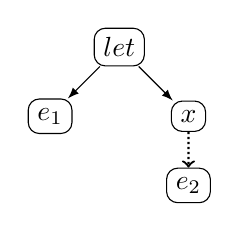
\begin{tikzpicture}[
      edge from parent/.style={draw,-latex},
      sibling distance=5em,
      level distance=2.5em,
      every node/.style = {shape=rectangle, rounded corners,
        draw, align=center,
        top color=white}]]
      \node {$\kw{let}$}
      child { node {$e_1$} }
      child { node {$\var{x}$}
        child { node {$e_2$} edge from parent[thick, densely dotted,->]
        }
      };
    \end{tikzpicture}
    \]
  \item \emph{Bound variable:} a variable under a binder, e.g.,
    $\elet {\estr{\text{hello}}} {x} {\ecat{\var
        x}{\estr{\text{world}}}}$
    % 
  \item A variable that is not bound is \emph{free}. A term with
    free-variables is \emph{open}, e.g., in
    $\elet{\estr{\text{hello}}}{x}{\ecat{\var x}{{{\var{y}}}}}$,
    $\var{y}$ is \emph{free}.
    % 
  \item A consequence of $e$ being well-typed is that it is
    \emph{closed}, i.e., $e$ has no free variable.
    % 
  \end{itemize}
\end{frame}



\subsection{Semantics}


\begin{frame}
  \frametitle{Semantics}
  The semantics of a programming language define what a program
  \emph{means}, i.e., how a program \emph{evaluates}.

  \bigskip

  The semantics of a programming language define ``dynamic''
  properties of the language, i.e., how programs ``move''.
  
\end{frame}

\begin{frame}
  \frametitle{Dynamics}
  \label{fr:value-e}

  The judgement ``$\valjudge{e}$'' states that $e$ is a value (i.e.,
  cannot be reduced further, it is the final result of a computation).
  % 
  % 
  % 
  It is inductively defined by the following two rules:
  \[
  \semrule{}
  {\,}
  {\valjudge{\enum{n}}}
  \qquad \qquad  \qquad
  \semrule{}
  {\,}
  {\valjudge{\estr{s}}}
  \]

  \bigskip
  \pause

  Are these values (i.e., does  $\valjudge{e}$ hold)?
  \begin{itemize}[<+->]
  \item $\estr{\text{hello}}$
  \item $\elet
    {\estr{\text{anotherstring}}}
    {y}
    {\eplus{y}{\etimes{\enum{1}}{\enum{2}}}}$
  \end{itemize}
\end{frame}



\begin{frame}
  \frametitle{Dynamics}
  
  Now, we define the actual semantics of language $\lggeE$, it is
  defined via judgement of the form: $\jtrans{e}{e'}$.
  % 
  
  \bigskip

  The transition judgement $\jtrans{e}{e'}$ between states is
  inductively defined by the following rules:

  \pause

  \[
  \semrule
  {\esemrulename{plval}}
  {n_1 + n_2 = n}
  {\jtrans{\eplus{\enum{n_1}}{\enum{n_2}}}{\enum{n}}}
  \]

  \pause

  \[
  \semrule
  {\esemrulename{pll}}
  {\jtrans{e_1}{e'_1}}
  {\jtrans{\eplus{e_1}{e_2}}{\eplus{e'_1}{e_2}}}
  \]
  
  \pause

  \[
  \semrule
  {\esemrulename{plr}}
  { \valjudge{e_1}
    \and
    \jtrans{e_2}{e'_2}}
  {\jtrans{\eplus{e_1}{e_2}}{\eplus{e_1}{e'_2}}}
  \]
  
\end{frame}


\begin{frame}
  \frametitle{Dynamics}

  \[
  \semrule
  {\esemrulename{tmval}}
  {n_1 \times n_2 = n}
  {\jtrans{\etimes{\enum{n_1}}{\enum{n_2}}}{\enum{n}}}
  \]

  \pause

  \[
  \semrule
  {\esemrulename{tml}}
  {\jtrans{e_1}{e'_1}}
  {\jtrans{\etimes{e_1}{e_2}}{\etimes{e'_1}{e_2}}}
  \]
  
  \pause

  \[
  \semrule
  {\esemrulename{tmr}}
  { \valjudge{e_1}
    \and
    \jtrans{e_2}{e'_2}}
  {\jtrans{\etimes{e_1}{e_2}}{\etimes{e_1}{e'_2}}}
  \]
  
\end{frame}


% \note{Exercise: give are the rules for $\etimes{e_1}{e_2}$?}


\begin{frame}
  \frametitle{Dynamics}
  \[
  \semrule
  {\esemrulename{catval}}
  {s_1 \concat s_2 = s}
  {\jtrans{\ecat{\estr{s_1}}{\estr{s_2}}}{\estr{s}}}
  \]


  \pause

  \[
  \semrule
  {\esemrulename{catl}}
  { \jtrans{e_1}{e'_1}}
  {\jtrans{\ecat{e_1}{e_2}}{\ecat{e'_1}{e_2}}}
  \]
  
  \pause

  \[
  \semrule
  {\esemrulename{catr}}
  {\valjudge{e_1}
    \and
    \jtrans{e_2}{e'_2}}
  {\jtrans{\ecat{e_1}{e_2}}{\ecat{e_1}{e'_2}}}
  \]
  

\end{frame}


\begin{frame}
  \frametitle{Dynamics}
  \begin{itemize}[<+->]
  \item  Call-by-name:
    \[
    \semrule
    {\esemrulename{letn}}
    {\,}
    {
      \jtrans{\elet{e_1}{x}{e_2}}{\subs{e_2}{e_1}{x}}}
    \]
  \item   Call-by-value:

    \[
    \semrule
    {\esemrulename{letm}}
    {\jtrans{e_1}{e'_1}}
    {
      \jtrans{\elet{e_1}{x}{e_2}}{\elet{e'_1}{x}{e_2}}}
    \]
    \[
    \semrule
    {\esemrulename{letv}}
    {\valjudge{e_1}}
    {
      \jtrans{\elet{e_1}{x}{e_2}}{\subs{e_2}{e_1}{x}}}
    \]
  \end{itemize}

  \bigskip 

  \pause

  Is call-by-name semantics equivalent to laziness
  (like the default behaviour in Haskell)?
  % 
  What kind of strategy does OCaml use?

\end{frame}

\begin{frame}
  \frametitle{Evaluation strategies}
  \begin{itemize}[<+->]
  \item \emph{Call-by-value:} arguments are evaluated to values
    \emph{before} being substituted in for variables. Main advantage:
    program's behavior (easy to determine when an expression is
    evaluated) and performance (each expression is evaluated at most
    once). Main disadvantage: evaluate everything, even if not needed.
    % 
  \item \emph{Call-by-name:} arguments are substituted without being
    computed. Main advantage: expressions whose value is never needed
    are not evaluated (evaluate as late as possible). Main
    disadvantage: requires a lot of memory.
    % 
  \item \emph{Call-by-need:} arguments are not evaluated until their
    values are needed, but once they are evaluated, the value is
    \emph{recorded} so that it can be reused. Main advantage:
    expressions are evaluated at most once.
    % 
    Good trade-off between CBV and CBN but harder to implement
    correctly and efficiently.
  \end{itemize}
\end{frame}

\begin{frame}
  \frametitle{Call-by-name vs.\ call-by-value}
  % 
  \label{fr:srategies-e}
  % 
  What are the advantages/disadvantages of call-by-name vs.\ call-by-value?


  \bigskip

  Consider the following programs:
  \begin{itemize}
  \item $\elet{\etimes{1852}{2017}}{x}{\eplus{\var{x}}{\var{x}}}$
  \item $\elet{\etimes{1852}{2017}}{x}{\eplus{\var{1}}{\var{x}}}$
  \item $\elet{\etimes{1852}{2017}}{x}{\eplus{\var{1}}{\var{13}}}$
  \end{itemize}
\end{frame}

\begin{frame}
  \frametitle{Examples}
  \label{fr:evaluate-e}

  Evaluate these $\lggeE$ phrases:
  \begin{itemize}
  \item $\ecat
    {\ecat
      {\estr{\text{hello}}}   
      {\estr{\text{world}}}
    }
    {\estr{\text{!}}}$
  \item $\etimes
    {\elen{\estr{\text{hello}}}}
    {\eplus{\enum{1}}{\elen{\estr{\text{world}}}}}$
    % 
  \item $\elet{\estr{\text{mystring}}}{x}{\etimes{\elen{\var{x}}}{\enum{0}}}$
    % 
  \item $\elet
    {\estr{\text{anotherstring}}}
    {\var{y}}
    {\eplus{\var{y}}{\etimes{\enum{1}}{\enum{2}}}}$
  \end{itemize}
\end{frame}

\begin{frame}
  \frametitle{Feedback from Week 19}
  \begin{itemize}
  \item Missed lectures: hard to catch up.
  \item How to break down expressions?
  \item Difficulty understanding binders (let)
  \item When to apply plr or pll, and why is there separate rules?
  \item Whether we should write ``$\valjudge{e}$'' judgements explicitly
  \item Syntax of substitutions
  \item Terminology rule names, gamma ($\Gamma$), tau ($\tau$)
  \item Full definitions of all languages will be on Moodle
  \end{itemize}
\end{frame}

\begin{frame}
  \frametitle{Recap}
  Judgements covered so far:
  
  \bigskip
  
  \begin{itemize}
    \setlength\itemsep{1.5em}
  \item \emph{Type system:}
    $\tyjudge{\var{x_1} : \tau_1, \ldots, \var{x_k}:\tau_k}{e}{\tau}$
    means that, assuming that variable $\var{x_i}$ has type $\tau_i$
    ($\forall 1 \leq i \leq k$), term $e$ has type $\tau$.
    % 
  \item \emph{Semantics (1):} $\valjudge{e}$ means that term $e$ is a \emph{value} (it
    cannot be evaluated further).
    % 
  \item \emph{Semantics (2):} $\jtrans{e}{e'}$ means that term $e$
    evaluate to term $e'$ (in one step).
  \end{itemize}
\end{frame}



%%% Local Variables:
%%% mode: latex
%%% TeX-master: "main"
%%% End:


\begin{frame}
  \label{fr:ite-e}
  \frametitle{Exercise}
  Add the following construct to language $\lggeE$:
  \[
  \site{e}{e_1}{e_2}
  \qquad\qquad \text{i.e.,} \quad
  \csite{e}{e_1}{e_2}
  \]
  
  \bigskip
  
  Think of what you will need to add wrt.\ syntax, types, and
  semantics.
\end{frame}




\subsection{Type safety}


\begin{frame}
  \frametitle{Type safety}
  \begin{itemize}
  \item We want \emph{type safe} programming languages
    % 
  \item i.e., certain kinds of mismatches cannot happen at runtime,
    e.g., we would like to avoid computation like: \texttt{``one'' == 123}.
    % 
  \item \emph{Type safety} expresses the \emph{coherence} between
    statics (types) and dynamics (semantics).
    % 
  \item A consequence of type safety is that evaluation cannot get stuck.
  \end{itemize}
\end{frame} 


\begin{frame}
  \frametitle{Type safety}\label{fr:ty-safety}

  Hereafter, we often write $\tyjudge{\,}{e}{\tau}$ for
  $\tyjudge{\varnothing}{e}{\tau}$.

  \bigskip 

  \pause

  \begin{theorem}[Type safety]
    \begin{enumerate}[<+->]
    \item If $\tyjudge{}{e}{\tau}$ and $\jtrans{e}{e'}$, then $\tyjudge{}{e'}{\tau}$.
    \item If $\tyjudge{}{e}{\tau}$, then either $\valjudge{e}$, or there exists $e'$ such that $\jtrans{e}{e'}$.
    \end{enumerate}
  \end{theorem}


  The first part of the theorem is often referred to as \emph{type
    preservation}, while the second part is referred to as
  \emph{progress}.
\end{frame}



\begin{frame}
  \frametitle{Runtime errors}

  Suppose we extend $\lggeE$ with a division operator:
  $\ediv{e_1}{e_2}$.
  

  \begin{itemize}
  \item  A natural typing rule is:
    \pause 
    \[
    \tyrule
    {\etyrulename{div}}
    {
      \tyjudge{\Gamma}{e_1}{\enum{}}
      \and
      \tyjudge{\Gamma}{e_2}{\enum{}}
    }
    {\tyjudge{\Gamma}{\ediv{e_1}{e_2}}{\enum{}}}
    % 
    \]

  \item    Main semantics rule: 
    \pause
    % 
    % 
    \[
    \semrule
    {\esemrulename{dval}}
    {n_1 \div n_2 = n}
    {\jtrans{\ediv{\enum{n_1}}{\enum{n_2}}}{\enum{n}}}
    \]

    
  \end{itemize}


  \pause 

  \bigskip

  \emph{Problem:} the expression $\ediv{\enum{3}}{\enum{0}}$ is
  \emph{well-typed}, yet ``\emph{stuck}''!
  % 
  
  % 
\end{frame}
\begin{frame}
  \frametitle{Runtime errors}

  \emph{Two possible solutions:}


  \bigskip

  \begin{itemize}[<+->]
  \item \emph{Enhanced the type-system}, so that no well-typed program
    may divide by zero.
    % 
  \item Add \emph{dynamic checks}, so that division-by-zero signals an error
    (of evaluation).
  \end{itemize}


  \pause
  
  \bigskip
  
  The first approach may rule out too many ``good'' programs.
  % 
  In general, we cannot predict \emph{statically} whether an
  expression will be non-zero when evaluated.
  

  \bigskip
  
  Hence, the second approach is generally preferred.
  % 
\end{frame}



\begin{frame}
  \frametitle{Checked vs. Unchecked errors}
  We need to distinguish between \emph{checked} and \emph{unchecked errors}.
  \bigskip
  \begin{description}
    \setlength\itemsep{2em}
    % 
  \item[Unchecked error:] ruled out by the type system. No run-time
    checking performed because the type system rules out the
    possibility of such errors arising.
    % 
  \item[Checked error:] not ruled out by the type system, hence
    run-time check \emph{must} occur, e.g., a zero divisor.
  \end{description}
\end{frame}



\begin{frame}
  \frametitle{Dealing with run-time error}
  % 
  \[
  \semrule
  {\esemrulename{dval}}
  {n_1 / n_2 = n \and n_2 > 0}
  {\jtrans{\ediv{\enum{n_1}}{\enum{n_2}}}{\enum{n}}}
  \]


  \pause
  
  \[
  \semrule
  {\esemrulename{dval}}
  {\,}
  {\jtrans{\ediv{\enum{n_1}}{\enum{0}}}{\eerror}}
  \]

  \pause

  \[
  \semrule
  {\esemrulename{dl}}
  {\jtrans{e_1}{e'_1}}
  {\jtrans{\ediv{e_1}{e_2}}{\ediv{e'_1}{e_2}}}
  \]

  \pause

  \[
  \semrule
  {\esemrulename{dr}}
  { \valjudge{e_1}
    \and
    \jtrans{e_2}{e'_2}}
  {\jtrans{\ediv{e_1}{e_2}}{\ediv{e_1}{e'_2}}}
  \]
  

  \pause
  \bigskip

  Note $\eerror$ is a new term in language $\lggeE$.
  \pause
  % 
  \[
    \tyrule
    {\etyrulename{err}}
    {
      \,
    }
    {\tyjudge{\Gamma}{\eerror}{\tau}}
      % 
    \]
  
\end{frame}


\begin{frame}
  \frametitle{Dealing with run-time error}
  
  How do we preserve \emph{type safety} with run-time errors?

  \bigskip
  \pause
  

  \emph{Idea:} use expression $\eerror$ (i.e., a \emph{checked} error)
  and define a judgement $\errjudge{e}$ stating that $e$ incurs a
  run-time checked error.
  % 
  % \[
  % \anorule
  % {\valjudge{e_1}}
  % {\errjudge{\ediv{e_1}{\enum{0}}}}
  % \quad
  % \anorule
  % {\errjudge{e_1}}
  % {\errjudge{\ediv{e_1}{e_2}}}
  % \quad
  % \anorule
  % {\valjudge{e_1}
  % \and \errjudge{e_2}}
  % {\errjudge{\ediv{e_1}{e_2}}}
  % \]

  \[
  \anorule{\,}{\errjudge{\eerror}}
  \]

  \begin{theorem}[Progress with error]
    % 
    If $\tyjudge{}{e}{\tau}$, then either $\errjudge{e}$, $\valjudge{e}$, or there
    exists $e'$ such that $\jtrans{e}{e'}$.
    % 
  \end{theorem}
\end{frame}


\begin{frame}
  \frametitle{Discussion}

  Do we need to update the \textbf{type preservation} statement?

  \pause
  \bigskip
  
  Can you think of other \textbf{examples} of checked / unchecked errors?
\end{frame}


%%% Local Variables:
%%% mode: latex
%%% TeX-master: "main"
%%% End:




% \begin{frame}{Questionnaires -- Feedback}
  
  \begin{itemize}[<+->]
    \setlength\itemsep{2em}
  \item What is a programming language?
    % 
  \item In your own words, explain what
    ``$\tyjudge{\varnothing}{e}{\tau}$'' means?
    % 
  \item Explain what
    ``$\jtrans{\eplus{\enum{3}}{\enum{5}}}{\enum{8}}$'' means, using
    your own words.
    % 
  \item Explain the following statement, using your own words:

    \begin{center}
      If $\tyjudge{}{e}{\tau}$ and $\jtrans{e}{e'}$, then $\tyjudge{}{e'}{\tau}$.
    \end{center}
    
    % 
  \item What does the following term evaluate to?
    \[ 
    {\eapp{\elam{\tau}{x}{\var{x}}}{\eplus{\enum{1}}{\var{x}}}}
    \]
  \end{itemize}

\end{frame}


%%% Local Variables:
%%% mode: latex
%%% TeX-master: "main"
%%% End:


\section{Higher-order functions}



\begin{frame}{Remember $\lggeE$?}
    \[
  \begin{array}{llclll}
    \TYPES & \tau & \Coloneqq & \enum{}  & \enum{} & \text{numbers}
    \\
           &&& \estr{} & \estr{} & \text{strings}
    \\
    \\  \pause
    % 
    \EXPS & e & \Coloneqq  & \var{x} & \var{x} & \text{variable}
    \\
           &&& \enum{n} & n & \text{numeral}
    \\
           &&& \estr{s} & \litstr{s} & \text{literal}
    \\
           &&& \eplus{e_1}{e_2} & e_1 {+} e_2 & \text{addition}
    \\
           &&& \etimes{e_1}{e_2} & e_1 {*} e_2 & \text{multiplication}
    \\
           &&& \ecat{e_1}{e_2} & e_1 \concat e_2 & \text{concatenate}
    \\
           &&& \elen{e} & \lvert e \rvert & \text{length}
    \\
           &&& \elet{e_1}{x}{e_2} & \clet{e_1}{x}{e_2} & \text{definition}
  \end{array}
  \]



%%% Local Variables:
%%% mode: latex
%%% TeX-master: "main"
%%% End:
 
\end{frame}


\begin{frame}
  \frametitle{Introduction}
  In $\lggeE$, to multiply a number by $2$, we can write:
  \[
  \clet{4}{x}{\etimes{\enum{2}}{\enum{x}}}
  \]
  whenever we want to double a number with have to ``redefine''
  the concept of doubling.


  \bigskip

  What if I don't want to write the concept of ``doubling'' several times in, e.g.,
  $(10\times2)+(4\times2)+(5\times2)$?
  
  \bigskip

  \pause

  \bigskip

  What concept(s) are we missing?
\end{frame}



\subsection{Syntax and types}

\begin{frame}[fragile]
  \frametitle{Language $\lggeEF$}

  \pause

  \[
  \begin{array}{llclll}
    \TYPES & \tau & \Coloneqq & \ldots {\color{gray} (\text{as in } \lggeE)}
    \\ 
           &&& \tyarr{\tau_1}{\tau_2}  & \tau_1 \rightarrow \tau_2 & \text{function}
    \\ 
    \\\pause
    \EXPS & e & \Coloneqq & \ldots {\color{gray} (\text{as in } \lggeE)}
    \\
           &&& \elam{\tau}{x}{e} & \clam{\tau}{x}{e} & \text{abstraction}
    \\
           &&& \eapp{e_1}{e_2} & \capp{e_1}{e_2} & \text{application}
  \end{array}
  \]

  \bigskip
  \pause

  In other programming languages:
\begin{lstlisting}
  (Object x) -> x.getClass() // Java

  \x -> x + 1                -- Haskell
\end{lstlisting}

  \pause

  \[
  \quad
  \begin{array}{ll}
    \text{Example:} \quad &
                            \cleta{\clam{\enum{}}{x}{\etimes{\var{x}}{\enum{2}}}}{double}
    \\
                          & 
                            \quad
                            \cletb
                            { 
                            \eplus{
                            \capp{\var{double}}{\enum{4}} 
                            }
                            {
                            \capp{\var{double}}{{\enum{10}}} 
                            }
                            }
  \end{array}
  \]
\end{frame}




\begin{frame}
  \frametitle{Statics}
  \[
  \tyrule
  {\eftyrulename{lam}}
  {
    \only<2->{
      \tyjudge{\Gamma, \var{x} : \tau_1}{e}{\tau_2}
    }
  }
  {\tyjudge{\Gamma}{\elam{\tau_1}{x}{e}}{\tyarr{\tau_1}{\tau_2}}}
  \]

  
  \bigskip


  \pause

  \pause
  
  \[
  \tyrule
  {\eftyrulename{ap}}
  {
    \only<4->{
      \tyjudge{\Gamma}{e_1}{\tyarr{\tau'}{\tau}}
    \and
      \tyjudge{\Gamma}{e_2}{\tau'}
    }
  }
  {
    \tyjudge{\Gamma}{\eapp{e_1}{e_2}}{\tau}
  }
  \]

\end{frame}


\subsection{Semantics}



\begin{frame}
  \frametitle{Examples}
  \label{fr:ef-types}
  Are these $\lggeEF$ programs well typed?


  {\footnotesize
    \begin{itemize}[<+->]
    \item $\elet{\clam{\enum{}}{x}{\etimes{\var{x}}{\var{x}}}}{sq}
      { 
        \eplus{
          \eapp{\var{sq}}{4} 
        }
        {
          \eapp{\var{sq}}{10} 
        }
      }$
      % 
    \item { $\elet{\clam{\enum{}}{x}{
            \clam{\enum{}}{y}{
              \etimes{\var x}{\var y}
            }
          }
        }{f}{
          \eapp
          {\eapp
            {\var{f}}
            {\enum{4}}
          }
          {\enum{4}}
        }
        $}
      
    \item $\elet{\clam{\enum{}}{x}{
          \eapp{\var f}{\eplus{\var{x}}{\enum{1}}}
        }
      }{f}{
        \eapp{\var{f}}{0}
      }$ 
    \end{itemize}
  }

\end{frame}



\begin{frame}
  \frametitle{Dynamics}

  First: define what a value is
  \pause

  \bigskip 
  \[
  \semrule
  {\efsemrulename{lam}}
  {\,}
  {\valjudge{\elam{\tau}{x}{e}}}
  \]
  
  \bigskip 
  \pause
  Second: define evaluation judgements
  \pause

  \[
  \semrule
  {\efsemrulename{ap}}
  {\jtrans{e_1}{e'_1}}
  {
    \jtrans{\eapp{e_1}{e_2}}{\eapp{e'_1}{e_2}}
  }
  \]

  \bigskip

  \pause

  \bigskip  

  We write $\jtransC{e_1}{e_n}$ if $\jtrans{e_1}{e_2}$,
  $\jtrans{e_2}{e_3}$, \ldots, $\jtrans{e_{n-1}}{e_n}$ for some
  terms $e_1$, \ldots, $e_{n-1}$.

\end{frame}

\begin{frame}
  \frametitle{Dynamics}

  \begin{itemize}[<+->]
  \item Call-by-name
    \[
    \semrule
    {\efsemrulename{apn}}
    {\,}
    {\jtrans{\eapp{\elam{\tau}{x}{e_1}}{e_2}}{\subs{e_1}{e_2}{x}}}
    \]
    % 
  \item Call-by-value

    \[
    \semrule
    {\efsemrulename{apr}}
    {\valjudge{e_1} 
      \and \jtrans{e_2}{e'_2}
    }
    {\jtrans{\eapp{e_1}{e_2}}{\eapp{e_1}{e'_2}}}
    \]

    
    \[
    \semrule
    {\efsemrulename{apl}}
    {\valjudge{e_2}}
    {\jtrans{\eapp{\elam{\tau}{x}{e_1}}{e_2}}{\subs{e_1}{e_2}{x}}}
    \]
  \end{itemize}

  \bigskip
  % 

  What are the differences between call-by-name and call-by-value?
\end{frame}

\begin{frame}
  \frametitle{Examples}
  \label{fr:evaluate-ef}
  Reduce the following expression (if they are typeable!):

  {\footnotesize
    \begin{itemize}[<+->]
    \item $\elet{\clam{\enum{}}{x}{\etimes{\var{x}}{\var{x}}}}{sq}
      { 
        \eplus{
          \eapp{\var{sq}}{4} 
        }
        {
          \eapp{\var{sq}}{10} 
        }
      }$
      % 
    \item $\elet{\clam{\enum{}}{x}{
          \clam{\enum{}}{y}{
            \etimes{\var x}{\var y}
          }
        }
      }{f}{
        \eapp
        {\var f}
        {\eapp
          {\enum{4}}
          {\enum{3}}
        }
      }$
      
    \item $\elet{\clam{\enum{}}{x}{
          \eapp{\var f}{\eplus{\var{x}}{\enum{1}}}
        }
      }{f}{
        \eapp{\var{f}}{0}
      }$ 
    \end{itemize}
  }

  \bigskip 




\end{frame}




\begin{frame}{Other examples}
  \label{fr:notype-ef}

  Type check then evaluate the following terms:
  % 
  % 
  \begin{itemize}
  \item {\small $ \eapp{
      \eapp{{\elam{\enum{}}{x}{\elam{\enum{}}{y}{\eplus{\var{x}}{\var{y}}}}}}
      {\enum{1}}
    }{\enum{2}}
    $}
    % 
  \item $\eapp
    {\elam{\tau}{x}{\eapp
        {\var{x}}
        {\var{x}}}
    }
    {\enum{2}}$
    % 
  \item $\eapp
    {\elam{\tau}{x}{\eapp
        {\var{x}}
        {\var{x}}}
    }
    {\elam{\tau'}{x}{\eapp
        {\var{x}}
        {\var{x}}}
    }$
    % 
  \end{itemize}

  \bigskip

  The same programs in concrete syntax:
  \begin{itemize}
  \item  $
    \capp{
      \capp{{\clam{\enum{}}{x}{\clam{\enum{}}{y}{{\var{x}+\var{y}}}}}}
      {\enum{1}}
    }{\enum{2}}
    $
  \item $\capp
    {\clam{\tau}{x}{\capp
        {\var{x}}
        {\var{x}}}
    }
    {\enum{2}}$
    % 
      \item $\capp
    {\clam{\tau}{x}{\capp
        {\var{x}}
        {\var{x}}}
    }
    {\clam{\tau'}{x}{\capp
        {\var{x}}
        {\var{x}}}
    }$
    % 
  \end{itemize}

  % 
  
\end{frame}


\begin{frame}
  \label{fr:eval-strat-ef}
  \frametitle{Evaluation strategies}
  Remember the difference between \emph{call-by-name} vs \emph{call-by-value} evaluations?
  
  \bigskip

  \begin{itemize}
  \item $\eapp{\elam{\enum{}}{x}{\eplus{\var{x}}{\var{x}}}}{e}$
    % $(\lambda \var{x} . \ \var{x} + \var{x}) \ e$
  \item $\eapp{\elam{\enum{}}{x}{\enum{42}}}{e}$
    
  \end{itemize}

  \bigskip

  Which evaluation strategy is the best for these terms?

\end{frame}

%%% Local Variables:
%%% mode: latex
%%% TeX-master: "main"
%%% End:


\section{Recursion}


% \begin{frame}
%   \frametitle{Housekeeping} 
%   \begin{itemize}[<+->]
%   \item Explain: ``if $\tyjudge{}{e}{\tau}$ and $\jtrans{e}{e'}$, then $\tyjudge{}{e'}{\tau}$''.
%     \begin{itemize}
%     \item If $e$ is well-typed and $e$ reduces to $e'$, then $e'$ is
%       also well-typed (and both $e$ and $e'$ have the same type).
%     \item This statement is also called \emph{type preservation} (cf.\ type safety,  slide~\ref{fr:ty-safety}).
%     \end{itemize}
%   \item Whiteboard pictures on Moodle $\implies$ ask on Piazza.
%   \item \LaTeX\ in the lectures $\implies$ too risky! 
%   \end{itemize}
% \end{frame}

\begin{frame}
  \frametitle{Introduction}

  \begin{center}
    {\large
      What is the \emph{expressive power} of the languages we have studied so far?
    }
  \end{center}

  \pause

  \bigskip  

  \begin{itemize}[<+->]
  \item We can specify the expressivity of a programming language by
    considering the set of computable functions it can represent.
    % 
  \item Most programming languages are \emph{universal}, i.e., Turing
    complete (meaning that they can be used to simulate a Turing
    machine).
    % 
  \item Hence, expressivity of programming languages is generally
    concerned with questions such as: can construct $C$ in language
    $L$ be simulated in language $L'$?
    % 
  \item For more on expressivity of programming languages beyond
    computational power, see, e.g.,
    \emph{``\href{https://www.sciencedirect.com/science/article/pii/016764239190036W}{On
        the expressive power of programming languages}''}, by Matthias
    Felleisen.
  \end{itemize} 

\end{frame}


% \note{In particular, what sort of recursive programs (or programs that
%   ``loop'' infinitely) can we write in the languages we have seen thus far?}

\begin{frame}
  \frametitle{Language \lggeT}
  % 
  \[
  \begin{array}{llclll}
    \TYPES & \tau & \Coloneqq & \tynat  & \tynat & \text{natural}
    \\
           &&& \tyarr{\tau_1}{\tau_2}  & \tau_1 \rightarrow \tau_2 & \text{function}
    \\
    \\ \pause
    \EXPS & e & \Coloneqq & \var{x} & \var{x} & \text{variable}
    \\
           &&& \ez &  \ez & \text{zero}
    \\
           &&& \esucc{e} &  \esucc{e} & \text{successor}
    \\
           &&& \elam{\tau}{x}{e} & \clam{\tau}{x}{e} & \text{abstraction}
    \\
           &&& \eapp{e_1}{e_2} & \capp{e_1}{e_2} & \text{application}
    \\
           &&& \eiter{e_0}{x}{e_1}{e} & \multicolumn{2}{c}{\citer{e_0}{x}{e_1}{e}}                                      
  \end{array}
  \]

  \pause

  We write $\bnum{3}$ for $\esucc{\esucc{\esucc{\ez}}}$.
\end{frame}

\begin{frame}
  \frametitle{Statics}
  % (same as $\lggeEF$)
  \[
  \tyrule
  {\ttyrulename{var}}
  {\,}
  {\tyjudge{\Gamma_1, \var{x}: \tau, \Gamma_2}{\var{x}}{\tau} }
  \]


  \pause 
  \bigskip

  \[
  \tyrule
  {\ttyrulename{nat}}
  {\,}
  {\tyjudge{\Gamma}{\ez}{\tynat}}
  \qquad\qquad\qquad
  \tyrule
  {\ttyrulename{num}}
  {\tyjudge{\Gamma}{{e}}{\tynat{}}}
  {\tyjudge{\Gamma}{\esucc{e}}{\tynat{}}}
  \]
\end{frame}




\begin{frame}
  \frametitle{Statics}
  
  \[
  \tyrule
  {\ttyrulename{lam}}
  {\tyjudge{\Gamma, \var{x} : \tau_1}{e}{\tau_2}}
  {\tyjudge{\Gamma}{\elam{\tau_1}{x}{e}}{\tyarr{\tau_1}{\tau_2}}}
  \]

  \pause

  \[
  \tyrule
  {\ttyrulename{ap}}
  {
    \tyjudge{\Gamma}{e_1}{\tyarr{\tau_1}{\tau}}
    \and
    \tyjudge{\Gamma}{e_2}{\tau_1}
  }
  {
    \tyjudge{\Gamma}{\eapp{e_1}{e_2}}{\tau}
  }
  \]


  \pause

  \bigskip

  \bigskip

  NB: this rules are the same as for Language $\lggeEF$.
\end{frame}



\begin{frame}
  \frametitle{Statics}
  \[
  \tyrule
  {\ttyrulename{ite}}
  {
    \tyjudge{\Gamma}{e}{\tynat}
    \and
    \tyjudge{\Gamma}{e_0}{\tau}
    \and
    \tyjudge{\Gamma, \var{x} : \tau}{e_1}{\tau}
  }
  {
    \tyjudge{\Gamma}{\eiter{e_0}{x}{e_1}{e}}{\tau}
  }
  \]

  \bigskip

  \pause
  
  Why do $e_0$ and $e_1$ need to have the same type?
  
\end{frame}


\begin{frame}
  \frametitle{Dynamics}
  \emph{Eager} semantics:
  \[
  \semrule{\tsemrulename{z}}
  {\,}
  {\valjudge{\ez}}
  \qquad \qquad  \qquad
  \semrule{\tsemrulename{s}}
  {\valjudge{e}}
  {\valjudge{\esucc{e}}}
  \]

  \[
  \semrule
  {\tsemrulename{lam}}
  {\,}
  {\valjudge{\elam{\tau}{x}{e}}}
  \]


\end{frame}


\begin{frame}
  \frametitle{Dynamics}
  
  % (same as $\lggeEF$)

  \[
  \semrule
  {\tsemrulename{ss}}
  {\jtrans{e}{e'}}
  {
    \jtrans{\esucc{e}}{\esucc{e'}}
  }
  \]

  \[
  \semrule
  {\tsemrulename{ap}}
  {\jtrans{e_1}{e'_1}}
  {
    \jtrans{\eapp{e_1}{e_2}}{\eapp{e'_1}{e_2}}
  }
  \]
\end{frame}

\begin{frame}
  \frametitle{Dynamics}
  %  (same as $\lggeEF$)

  \[
  \semrule
  {\tsemrulename{lan}}
  {\valjudge{e_1} 
    \and \jtrans{e_2}{e'_2}
  }
  {\jtrans{\eapp{e_1}{e_2}}{\eapp{e_1}{e'_2}}}
  \]

  \[
  \semrule
  {\tsemrulename{lav}}
  {\valjudge{e_2}}
  {\jtrans{\eapp{\elam{\tau}{x}{e_1}}{e_2}}{\subs{e_1}{e_2}{x}}}
  \]
\end{frame}

\begin{frame}
  \frametitle{Dynamics (iterator)}
  

  \begin{itemize}[<+->]
  \item Evaluate the parameter
    \[
    \semrule
    {\tsemrulename{rin}}
    {\jtrans{e}{e'}}
    {
      \jtrans{\eiter{e_0}{x}{e_1}{e}}{\eiter{e_0}{x}{e_1}{e'}}
    }
    \]
    % 
  \item Case if zero 
    \[
    \semrule
    {\tsemrulename{r0}}
    {\,}
    {
      \jtrans{\eiter{e_0}{x}{e_1}{\ez}}{e_0}
    }
    \]
  \item Case if strictly positive
    \[
    \semrule
    {\tsemrulename{rs}}
    {\valjudge{{e}}}
    {
      \jtrans{\eiter{e_0}{x}{e_1}{\esucc{e}}}{\subs{e_1}{{\eiter{e_0}{x}{e_1}{{e}}}}{x}}
    }
    \]
  \end{itemize}


  NB: $\eiter{e_0}{x}{e_1}{e}$ stands for ${\citer{e_0}{x}{e_1}{e}}$     
\end{frame}

\begin{frame}
  \frametitle{Alpha equivalence ($\aeq$)}
  \begin{itemize}[<+->]
  \item Two programs are \emph{$\alpha$-equivalent} if they are
    identical up to the choice of \emph{bound} variables.
    % 
    \pause
    \[
    \elam{\tynat}{x}{\esucc{\var{x}}} \aeq   \elam{\tynat}{y}{\esucc{\var{y}}}
    \]

    \pause


    \[
    \esucc{\var{x}} \naeq \esucc{\var{y}}
    \]
    
  \end{itemize}
\end{frame}

\begin{frame}
  \frametitle{Alpha equivalence ($\aeq$)}
  \begin{itemize}
  \item \emph{Bound} variables can be renamed \emph{consistently}
    without changing the meaning of a program.
    \[
    \begin{array}{c}
      \elam{\tyarr{\tynat}{\tynat}}{x_1}{
      \elam{\tynat}{x_2}{
      \eapp
      {\var{x_1}}
      {\var{x_2}}
      }
      }
      \\
      \pause 
      \qquad
      \aeq
      \elam{\tyarr{\tynat}{\tynat}}{y_1}{
      \elam{\tynat}{y_2}{
      \eapp
      {\var{y_1}}
      {\var{y_2}}
      }
      }
      \\
      \pause
      \qquad
      \naeq
      \elam{\tyarr{\tynat}{\tynat}}{y_1}{
      \elam{\tynat}{y_2}{
      \eapp
      {\underline{\var{y_2}}}
      {\underline{\var{y_1}}}
      }
      }
    \end{array}
    \]
    \pause
  \item It's helpful to rename bound variables so that they are all
    \emph{distinct}, e.g.,
    \[
    \begin{array}{c}
      \eapp
      {\elam{\tau}{x}{{\var{x}}}}
      {\elam{\tau'}{x}{\esucc{\var{x}}}}
      \\ \qquad
      \pause
      \aeq
      \eapp
      {\elam{\tau}{x}{{\var{x}}}}
      {\elam{\tau'}{y}{\esucc{\var{y}}}}
    \end{array}
    \]
    
  \end{itemize}
\end{frame}


\begin{frame}
  \frametitle{Substitution}
  {\Large
    \[
    \subs{e_1}{e_2}{x}
    \]
  }
  \pause
  \begin{itemize}[<+->]
  \item Substitution is the process of ``plugging in'' an object
    ($e_2$) for the variable ($\var{x}$) in a program ($e_1$).
    % 
  \item Only the \emph{free} occurrences of variable $\var{x}$ should
    be replaced!
  \item Example: if
    \[ 
    e_1 = \eapp{\elam{\tynat}{x}{\esucc{\var{x}}}}{\underline{\var{x}}}
    \]
    \pause
    then 
    \[
    \subs{e_1}{\ez}{x} = 
    \pause
    \eapp{\elam{\tynat}{x}{\esucc{\var{x}}}}{\ez}
    \]
  \end{itemize}
  % 
  \pause
  NB: $ \eapp{\elam{\tynat}{x}{\esucc{\var{x}}}}{\underline{\var{x}}} 
  \aeq  \eapp{\elam{\tynat}{y}{\esucc{\var{y}}}}{\underline{\var{x}}} $
\end{frame}


\begin{frame}{Exercises}
  \label{fr:define-t}
  % 
  In $\lggeT$, implement the following functions:
  \begin{itemize}[<+->]
  \item Successor ($\tynat{} \rightarrow \tynat$): $\text{succ} \defi \clam{\tynat{}}{x}{{\color{red} ??}}$
  \item Doubling ($\tynat{} \rightarrow \tynat$): {\color{red} ??}
  \item Addition ($\tynat{} \rightarrow \tynat \rightarrow \tynat$): 
    $\text{add} \defi \clam{\tynat{}}{x}{\clam{\tynat{}}{y}{ {\color{red} ??} }}$
  \item Multiplication ($\tynat{} \rightarrow \tynat \rightarrow \tynat$): {\color{red} ??}
    % 
    % 
  \end{itemize}
   
  % \pause
  % \bigskip 
  
  % Using complex data types (see further chapters):
  % \begin{itemize}
  % \item Predecessor ($\tynat{} \rightarrow \tynat$): {\color{red} ??} (add product types to $\lggeT$)
  % \item Subtraction ($\tynat{} \rightarrow \tynat \rightarrow \tynat$): {\color{red} ??}
  % \end{itemize}
\end{frame}

% Add: \x \y . iter x { z -> y | v -> s(v)}
% Doubling: \x . iter x {z -> z | v -> s(s(v))}
% Multiply: \x \y . iter x {z -> z | v -> add(y,v)}
% Predecessor: \x . pl(iter x {z -> <z,z> | v -> <pr . v, s(pr . v)>})
% Subtraction: \x \y . iter x {z -> y | v -> pred(v)}




% \begin{frame}
%   \frametitle{Housekeeping}
%   \begin{itemize}[<+->]
%   \item What does the following term evaluate to
%     \[
%     \eapp{\elam{\tynat}{x}{\var{x}}}{\esucc{{\var{x}}}}
%     \]
%   \item Is language $\lggeT$ using Peano numbers? Yes, $\lggeT$ is
%     based on Godel's system T (1958), which includes Peano
%     axioms/numbers.
%   \end{itemize}
% \end{frame}
\begin{frame}
  \frametitle{Expressivity of $\lggeT$}
  \begin{itemize}
  \item Language $\lggeT$ provides a mechanism called \emph{primitive
      recursion} (which we used to define arithmetic operations).
    % 
  \item Primitive recursion can characterise the \emph{inductive}
    nature of the natural numbers.
    % 
  \item In $\lggeT$, we can only define \emph{total recursive
      functions} on the natural numbers (functions that \emph{always} return
    something).
    %  
  \item This inductive natures implies that every program comes with a
    proof of its \emph{termination} (we always ``bottom out'' using the
    induction principle).
    % 
  \item To obtain Turing completeness, we need a \emph{partial
      recursive} language (where some programs may not terminate).
  \end{itemize}
\end{frame}



% \separator{Examinable material for 2018 \emph{ends} here.}


\begin{frame}
  \frametitle{Y-Combinator}
  An option to express \emph{general recursion}\footnote{i.e.,
    allowing for partial functions.} is to introduce the $Y$
  combinator.
  
  \bigskip
  Its type is
  \[
  Y : (\tau \rightarrow \tau) \rightarrow \tau
  \]
  

  \pause

  Additional semantic rule:
  \[
  \semrule
  {\tsemrulename{y}}
  {\,}
  {
    \jtrans{Y f}{ f(Y f)}
  }
  \]

  \pause
  \bigskip
 
  NB: in the \emph{untyped} lambda-calculus, it can be expressed as
  \[
  Y \defi \lambda f  .\ (\lambda x . f (x \ x))  \ (\lambda x . f (x \ x))
  \]

  Exercise: try to find a type for that term!
\end{frame}

\separator{Examinable material for 2020 ends here.}

%%% Local Variables:
%%% mode: latex
%%% TeX-master: "main"
%%% End:

%  LocalWords:  computable expressivity Examinable
 % strict minimum

\section{Data types}

\begin{frame}
  \frametitle{Introduction}

  So far, we have only considered two sorts of data types: $\enum{}$
  and $\estr{}$.
  % 
  Most programming languages allow ``\emph{complex}'' types.

  \bigskip

  Examples?
  
\end{frame}


\note{This part is adapted from Chapters 10 and 11 of PFPL.}


\subsection{Binary product}

\begin{frame}
  \frametitle{Syntax}

  A language with binary \emph{product}.

  \[
  \begin{array}{llclll}
    \TYPES & \tau & \Coloneqq &  \ldots {\color{gray} (\text{as in } \lggeEF)}
    \\
    % &&& \tyunit  & \tyunit & \text{nullary product}
    % \\
           &&& \typrod{\tau_1}{\tau_2} & \tau_1 {\times} \tau_2 & \text{binary product} 
    \\
    \\
    \EXPS & e & \Coloneqq &  \ldots {\color{gray} (\text{as in } \lggeEF)}
    \\
    % &&& \etriv & \ctriv & \text{null tuple}
    % \\
           &&& \epair{e_1}{e_2} & \cpair{e_1}{e_2}  & \text{ordered pair}
    \\
           &&& \eprl{e} & \cprl{e} & \text{left projection}
    \\
           &&& \eprr{e} & \cprr{e} & \text{right projection}
  \end{array}
  \]
\end{frame}


\begin{frame}
  \frametitle{Statics}
  % \[
  % \tyrule
  % {\etyrulename{u}}
  % {\,}
  % {\tyjudge{\Gamma}{\etriv}{\tyunit} }
  % \]
  \[
  \tyrule
  {\etyrulename{prod}}
  {\tyjudge{\Gamma}{e_1}{{\tau_1}}
    \and
    \tyjudge{\Gamma}{e_2}{{\tau_2}}
  }
  {\tyjudge{\Gamma}{\epair{e_1}{e_2}}{\typrod{\tau_1}{\tau_2}}}
  \]
  \pause
  \bigskip
  \[
  \tyrule
  {\etyrulename{pl}}
  {\tyjudge{\Gamma}{e}{\typrod{\tau_1}{\tau_2}}
  }
  {\tyjudge{\Gamma}{\eprl{e}}{\tau_1}} 
  \qquad\qquad\quad
  \tyrule
  {\etyrulename{pr}}
  {\tyjudge{\Gamma}{e}{\typrod{\tau_1}{\tau_2}}
  }
  {\tyjudge{\Gamma}{\eprr{e}}{\tau_2}} 
  \]
\end{frame}



\begin{frame}
  \frametitle{Examples}
  Find the type for the following terms, if possible.

  \begin{itemize}
  \item $\epair{\enum{2}}{\estr{\text{hello}}}$
  \item $\eprl{\epair{\enum{2}}{\estr{\text{hello}}}}$
  \item $\elam{\typrod{\enum{}}{\estr{}}}{x}{\epair{\eprr{x}}{\eprl{x}}}$
  \item $\eapp{\elam{\typrod{\enum{}}{\estr{}}}{x}{\epair{\eprr{x}}{\eprl{x}}}}{\etriv}$
  \end{itemize}

\end{frame}


\begin{frame}
  \frametitle{Dynamics (lazy)}
  
  \[
  % \semrule{}
  % {\,}
  % {\valjudge{\etriv}}
  % \qquad\qquad\quad
  \semrule{}
  {\,
    % \valjudge{e_1} \and \valjudge{e_2}
  }
  { \valjudge{\epair{e_1}{e_2}} }
  \]
  

  \[
  \semrule
  {\esemrulename{pll}}
  {\jtrans{e}{e'}}
  {\jtrans{\eprl{e}}{\eprl{e'}}}
  \qquad\qquad\quad
  \semrule
  {\esemrulename{plr}}
  {\jtrans{e}{e'}}
  {\jtrans{\eprr{e}}{\eprr{e'}}}
  \]

  \[
  \semrule
  {\esemrulename{pll}}
  {\,}
  {\jtrans{\eprl{\epair{e_1}{e_2}}}{{e_1}}}
 \qquad\qquad
  \semrule
  {\esemrulename{plr}}
  {\,}
  {\jtrans{\eprr{\epair{e_1}{e_2}}}{{e_2}}}
  \]
\end{frame}


\begin{frame}
  \frametitle{Examples}
  Evaluate the following terms, if they can be assigned a type.
  % 
  \begin{itemize}
  \item $\epair{\enum{2}}{\estr{\text{hello}}}$
  \item $\eprl{\epair{\enum{2}}{\estr{\text{hello}}}}$
  \item $\elam{\typrod{\enum{}}{\estr{}}}{x}{\epair{\eprr{x}}{\eprl{x}}}$
  \item $\eapp{\elam{\typrod{\enum{}}{\estr{}}}{x}{\epair{\eprr{x}}{\eprl{x}}}}{\etriv}$
  \end{itemize}

\end{frame}



\subsection{Nullary and binary sum}

\begin{frame}
  \frametitle{Syntax}

  A language with nullary and binary \emph{sum}.

  \[
  \begin{array}{llclll}
    \TYPES & \tau & \Coloneqq &  \ldots {\color{gray} (\text{as in } \lggeEF)}
    % \\
    %        &&& \tyvoid  & \tyvoid & \text{nullary sum}
    \\
           &&& \tysum{\tau_1}{\tau_2} & \tau_1 {+} \tau_2 & \text{binary sum} 
    \\
    \\
    \EXPS & e & \Coloneqq &  \ldots {\color{gray} (\text{as in } \lggeEF)}
    \\
    %        &&& \eabort{\tau}{e} & \cabort{e} & \text{abort}
    % \\
           &&& \einl{\tau_1}{\tau_2}{e} & \cinl{e}  & \text{left injection}
    \\
           &&&  \einr{\tau_1}{\tau_2}{e} & \cinr{e}  & \text{right injection}
    \\
           &&& \ecase{e}{x_1}{e_1}{x_2}{e_2} & \text{\tiny[see below]} & \text{case analysis}
  \end{array}
  \]

  Concrete form for case analysis: $\ccase{e}{x_1}{e_1}{x_2}{e_2}$
\end{frame}


\begin{frame}
  \frametitle{Statics}

  % \[
  % \tyrule
  % {\etyrulename{u}}
  % {\tyjudge{\Gamma}{e}{\tyvoid}}
  % {\tyjudge{\Gamma}{\eabort{\tau}{e}}{\tau}}
  % \]

  \[
  \tyrule
  {\etyrulename{inl}}
  {
    \tyjudge{\Gamma}{e_1}{{\tau_1}}
  }
  {\tyjudge{\Gamma}{\einl{\tau_1}{\tau_2}{e}}{\tysum{\tau_1}{\tau_2}}}
  \]

  \[
  \tyrule
  {\etyrulename{inr}}
  {
    \tyjudge{\Gamma}{e_2}{{\tau_2}}
  }
  {\tyjudge{\Gamma}{\einr{\tau_1}{\tau_2}{e}}{\tysum{\tau_1}{\tau_2}}}
  \]


  \[
  \tyrule
  {\etyrulename{cs}}
  {
    \tyjudge{\Gamma}{e}{\tysum{\tau_1}{\tau_2}}
    \and
    \tyjudge{\Gamma, \var{x_1}: {\tau_1}}{e_1}{\tau}
    \and
    \tyjudge{\Gamma, \var{x_2}: {\tau_2}}{e_2}{\tau}
  }
  {
    \tyjudge{\Gamma}
    {
      \ecase{e}{x_1}{e_1}{x_2}{e_2}
    }
    {\tau}
  }
  \]

  \bigskip

  Can we relax rule [\etyrulename{cs}] so that branches have
  different types?

\end{frame}

\begin{frame}
  \frametitle{Dynamics (eager)}

  
  \[
  \semrule{}
  {\valjudge{e}}
  {\valjudge{\einr{\tau_1}{\tau_2}{e}}}
  \qquad\qquad\quad
  \semrule{\etyrulename{ir}}
  {\jtrans{e}{e'}}
  {\jtrans{\einr{\tau_1}{\tau_2}{e}}{\einr{\tau_1}{\tau_2}{e'}}}
  \]
  



  \[
  \semrule{\etyrulename{inl}}
  {\valjudge{e}}
  {
    \jtrans{\ecase{\einl{\tau_1}{\tau_2}{e}}{x_1}{e_1}{x_2}{e_2}}
    {\subs{e_1}{e}{x_1}}
  }
  \]

  \[
  \semrule{\etyrulename{inr}}
  {\valjudge{e}}
  {
    \jtrans{\ecase{\einr{\tau_1}{\tau_2}{e}}{x_1}{e_1}{x_2}{e_2}}
    {\subs{e_2}{e}{x_2}}
  }
  \]


  \bigskip
  

  Anything missing?
\end{frame}


\subsection{Discussion}

\begin{frame}
  \frametitle{Constructors}
  We distinguish two sorts of type \emph{constructors}
  \begin{itemize}
  \item \emph{Introduction} forms construct a new term of the expected
    type, e.g., $\epair{e_1}{e_2}$ for binary products and
    $\einl{\tau_1}{\tau_2}{e_1}$ for binary sums.
    % 
  \item \emph{Elimination} forms destruct a term of a give type into a
    ``smaller'' type, e.g., $\eprl{e}$ for binary sums and
    $\ecase{e}{x_1}{e_1}{x_2}{e_2}$ for binary sums.
  \end{itemize}

  \bigskip

  Any other example?
  
\end{frame}


\begin{frame}
  \frametitle{Exercises}
  Define the functions (in $\lggeEF$ with pairs and sums) that meet
  the following specification:
  \begin{itemize}
  \item A function that \emph{adds} the content of the pairs:
    $\text{addpair} \defi \clam{\typrod{\enum{}}{\enum{}}}{x}{\eplus{\cprl{x}}{\cprr{x}}}$. Observe that $\text{addpair}$ has type $\tyarr{\typrod{\enum{}}{\enum{}}}{\enum{}}$.
    % 
  \item A function that \emph{flips} the content of a pair (e.g.,
    $\cpair{1}{2}$ becomes $\cpair{2}{1}$)
    % 
  \item A function that takes \emph{either} a string or a number as a
    parameter and returns the length of the string if the argument is
    a string, or the square of the argument if it's a number.
    % 
  \item A function of type
    $\tyarr{\tysum{\tau_1}{\tau_1}}{\tyarr{\tau_2}{\tyarr{\tau_2}{\tau_2}}}$,
    or, equivalently,
    $ (\tau_1 {+} \tau_1) \rightarrow \tau \rightarrow \tau
    \rightarrow \tau$
    (three parameters), which returns its second argument if its first
    is $\cinl{e}$ and returns its third argument if its first is
    $\cinr{e}$ (for some $e$).
  \end{itemize}
\end{frame}



\begin{frame}
  \frametitle{Applications and generalisations}
  \begin{itemize}
  \item Records 
  \item Labelled variants
  \item Optional types with binary sums
  \item Booleans
  \item $n$-ary sums and products
  \end{itemize}
\end{frame}


%%% Local Variables:
%%% mode: latex
%%% TeX-master: "main"
%%% End:


\section{Polymorphism}

\begin{frame}[fragile,fragile]
  \frametitle{Introduction}
  Take a language such as $\lggeEF$ with base types $\enum{}$ and
  $\estr{}$ and product types.
  
  Can we define \emph{one} function which takes a triple (e.g.,
  $\cpair{a}{\cpair{b}{c}}$) and returns the middle element (i.e., $b$)?

  % \bigskip

  \[
  \elam{\typrod{\enum{}}{\typrod{\enum{}}{\enum{}}}}{x}{ \eprl{\eprr{\var x}}}
  \]
  
  \begin{lstlisting}[language=Haskell]
-- Haskell
middle :: (t1,(t2,t3)) -> t2
middle (x,(y,z)) = y
\end{lstlisting}
  
\begin{lstlisting}[language=Java]
// Java
// (assume class Pair<T, V> exists)
public <S> S getMiddle(Pair<T,Pair<S,V>> triple){
  return triple.getRight().getLeft();
}
\end{lstlisting}

\bigskip
  
  More examples?
  
\end{frame}



\begin{frame}
  \frametitle{Polymorphicity}
  \begin{itemize}
  \item The term \emph{polymorphism} refers to a range of language mechanisms
    that allow a single part of a program to be used with different
    types in different contexts.
    % 
  \item The languages we have considered so far are all
    \emph{monomorphic} in that every expression has at most \emph{one}
    type (given the types of its free variables).
    % 
  \item \emph{Overloading} is a form of ``ad-hoc polymorphism''. It
    associates a single function symbol with many implementations.
    The compiler chooses an appropriate implementation for each
    application of the function, based on the types of the arguments.
  \end{itemize}
\end{frame}

\subsection{Syntax}

\begin{frame}
  \frametitle{Language $\lggeF$}
  \[
  \begin{array}{llclll}
    \TYPES & \tau & \Coloneqq & \tvar{t} & \tvar{t} & \text{type variable}
    \\ 
           &&& \tyarr{\tau_1}{\tau_2}  & \tau_1 \rightarrow \tau_2 & \text{function}
    \\
           &&& \tyall{t}{\tau} & \ctyall{t}{\tau} & \text{polymorphic}
    \\
    \\
    \EXPS & e & \Coloneqq & \var{x} & \var{x} & \text{variable}
    \\
           &&& \elam{\tau}{x}{e} & \clam{\tau}{x}{e} & \text{abstraction}
    \\
           &&& \eapp{e_1}{e_2} & \capp{e_1}{e_2} & \text{application}
    \\
           &&& \eLAM{t}{e} & \cLAM{t}{e} & \text{type abstraction}
    \\
           &&& \eAPP{\tau}{e} & \cAPP{\tau}{e} & \text{type application}
  \end{array}
  \]
\end{frame}


\begin{frame}
  \frametitle{Exercises}
  \begin{itemize}
  \item Define the identify function ($\texttt{id}(x) = x$)
  \item Define a polymorphic function to compose function together ($f \circ g = f(g(x))$)
  \item Any more ``standard'' polymorphic functions?
  \end{itemize}
\end{frame}

% L(T) . \x:t . x
% L(T1) . L(T2) . L(T2) \f:T2->T3 \g:T1->T2 = f(g(x))


\subsection{Statics}

\begin{frame}
  \frametitle{Judgements}

  Two judgement forms and two kinds of environments, the hypotheses in
  $\Delta$ have the form $\tvar{t} \ \typeok$, where $\tvar{t}$ is a
  variable of sort $\TYPES$ and the hypotheses in $\Gamma$ have the
  form $\var{x} : \tau$, where $\var{x}$ is a variable of sort $\EXPS$.

  \bigskip

  \begin{itemize}
  \item   {\Huge
      $    
      {\typejudge{\Delta}{\tau}}
      $   
    }

    says that the type $\tau$ is well-formed, under the hypotheses in $\Delta$

    \bigskip

  \item   {\Huge
      $    
      {\tyFjudge{\Delta}{\Gamma}{e}{\tau}}
      $   
    }
    
    says that the expression $e$ has type $\tau$, under  the hypotheses in $\Delta$ and $\Gamma$
  \end{itemize}
\end{frame}



\note{As usual, we write $\varnothing$ for the empty context $\Delta$ or $\Gamma$}


\begin{frame}
  \frametitle{Well-formed types}
 \[
  \tyrule
  {}
  {\,}
  {\typejudge{\Delta, \tvar{t} \ \typeok , \Delta_2}{\tvar{t}} }
  \]

  
  \[
  \tyrule
  {}
  {
    \typejudge{\Delta}{\tau_1}
    \and
    \typejudge{\Delta}{\tau_2}
  }
  {\typejudge{\Delta}{\tyarr{\tau_1}{\tau_2}} }
  \]

  
  \[
  \tyrule
  {}
  {
    \typejudge{\Delta, \tvar{t} \ \typeok }{\tau}
  }
  {\typejudge{\Delta}{\tyall{t}{\tau}} }
  \]
  
\end{frame}

\begin{frame}
  \frametitle{Examples}
  Are these types well-formed?
  \begin{itemize}
  \item $\tyall{t}{\tyarr{\tvar t}{\tvar t}}$
  \item $\tyall{t_1}{\tyall{t_2}{\tvar{t_1}}}$
  \item $\tyall{t_1}{\tyall{t_2}{\tyarr{\tvar{t_2}}{\tvar{t_1}}}}$
  \end{itemize}
\end{frame}


\begin{frame}
  \frametitle{Typing judgements (1)}
  \[
  \tyrule
  {\ftyrulename{var}}
  {\,}
  {\tyFjudge{\Delta}{\Gamma_1, \var{x}: \tau, \Gamma_2 }{\var{x}}{\tau} }
  \]


  \[
  \tyrule
  {\ftyrulename{lam}}
  {\tyFjudge{\Delta}{\Gamma, \var{x} : \tau_1}{e}{\tau_2}}
  {\tyFjudge{\Delta}{\Gamma}{\elam{\tau_1}{x}{e}}{\tyarr{\tau_1}{\tau_2}}}
  \]

  \[
  \tyrule
  {\ftyrulename{ap}}
  {
    \tyFjudge{\Delta}{\Gamma}{e_1}{\tyarr{\tau_1}{\tau_2}}
    \and
    \tyFjudge{\Delta}{\Gamma}{e_2}{\tau_2}
  }
  {
    \tyFjudge{\Delta}{\Gamma}{\eapp{e_1}{e_2}}{\tau_2}
  }
  \]

\end{frame}


\begin{frame}
  \frametitle{Typing judgements (2)}
  

  \[
  \tyrule
  {\ftyrulename{tlam}}
  {\tyFjudge{\Delta, \tvar{t} \ \typeok}{\Gamma}{e}{\tau}}
  {
    \tyFjudge{\Delta}{\Gamma}{\eLAM{t}{e}}{\tyall{t}{\tau}}
  }
  \]


  \[
  \tyrule
  {\ftyrulename{tap}}
  {
    \typejudge{\Delta}{\tau}
    \and
    \tyFjudge{\Delta}{\Gamma}{e}{\tyall{t}{\tau'}}
  }
  {
    \tyFjudge{\Delta}{\Gamma}{\eAPP{\tau}{e}}{\tsubs{\tau'}{\tau}{t}}
  }
  \]

\end{frame}

\begin{frame}
  \frametitle{Examples}
  Assuming we have product types, do these expression have a type?
  \begin{itemize}
  \item $\eLAM{t}{\elam{\tvar{t}}{x}{\var x}}$
  \item $\eLAM{t}{\elam{\typrod{\tvar{t}}{\typrod{\tvar{t}}{\tvar{t}}}}{x}{ \eprl{\eprr{\var x}}}}$
  \item Check for the solution of $f \circ g$
  \end{itemize}
\end{frame}

% let as lambda => (\id . <id "hello", id 123>) (\x . x)


\subsection{Semantics}

\begin{frame}
  \frametitle{Dynamics}
  \textbf{Call-by-name} semantics
  \[
  \semrule
  {\fsemrulename{lam}}
  {\,}
  {\valjudge{\elam{\tau}{x}{e}}}
  \]

  \[
  \semrule
  {\fsemrulename{tlam}}
  {\,}
  {\valjudge{\eLAM{t}{e}}}
  \]

\end{frame}

\begin{frame}
  \frametitle{Dynamics}
  \[
  \semrule
  {\fsemrulename{ap}}
  {\jtrans{e_1}{e'_1}}
  {
    \jtrans{\eapp{e_1}{e_2}}{\eapp{e'_1}{e_2}}
  }
  \]

  \[
  \semrule
  {\fsemrulename{lav}}
  {\,}
  {\jtrans{\eapp{\elam{\tau}{x}{e_1}}{e_2}}{\subs{e_1}{e_2}{x}}}
  \]
\end{frame}




\begin{frame}
  \frametitle{Dynamics}
  \[
  \semrule
  {\fsemrulename{ap}}
  {\,}
  {
    \jtrans
    {\eAPP{\tau}{\eLAM{t}{e}}}
    {\tsubs{e}{\tau}{t}}
  }
  \]

  \[
  \semrule
  {\fsemrulename{lav}}
  {\jtrans{e}{e'}}
  {
    \jtrans
    {\eAPP{\tau}{e}}
    {\eAPP{\tau}{e'}}
  }
  \]
\end{frame}


\begin{frame}
  \frametitle{Expressivity of $\lggeF$}
  Product and sum type can be expressed with the construct
  of $\lggeF$!
  %
  See Chapter 16.2 of PFPL.
\end{frame}

%%% Local Variables:
%%% mode: latex
%%% TeX-master: "main"
%%% End:




\section{Mutable variables}



\begin{frame}
  \frametitle{Introduction}

  All the languages we have seen so far belong to the realm of
  \emph{functional} programming language.
  % 
  In particular, in these languages variables are \emph{immutable}.

  \bigskip

  In this lecture, we study language $\lggeW$, a small \emph{imperative}
  programming language with \emph{mutable} variables
\end{frame}

\begin{frame}
  \frametitle{Language \lggeW}
  % 
  % 
  Let $\VARS$ be a set of variables,
  % 
  $n \in \naturals$, $t \in \{\ktrue,\kfalse\}$, and $\var{x} \in \VARS$.
  % 
  \[
  \begin{array}{llclll}
    \AEXPS & a & \Coloneqq & n \bnfsep \var{x} \bnfsep a_1 + a_2 \bnfsep a_1 * a_2 
    & \text{Arith.\ exp.\ } 
    \\
    \\
    \BEXPS & b  & \Coloneqq 
                           & t \bnfsep b_1 \land b_2 \bnfsep \neg b \bnfsep a_1 \leq a_2 
    & \text{Bool.\ exp.\ }
    \\
    \\
    \STMTS  & s & \Coloneqq & \sskip & \text{no nop}
    \\
           &&& {s_1 ; s_2} & \text{sequence}
    \\
           &&& \cset{x}{a} & \text{assign}
    \\
           &&&  \csite{b}{s_1}{s_2} & \text{if-then-else}
    \\
           &&&  \cwhile{b}{s} & \text{while}
  \end{array}
  \]
\end{frame}



\begin{frame}
  \frametitle{Dynamics -- big step semantics}
  % 
  $\Sigma$ represents the memory, formally, it's a map
  $\Sigma : \VARS \rightarrow \naturals$ from variable names to
  (positive) integers.
  % 
  \[
  \semrule
  {}
  {\,}
  {\bsjudge{\wconf{\Sigma}{n}}{n}}
  \qquad\qquad
  \semrule
  {}
  {\,}
  {\bsjudge{\wconf{\Sigma}{\var{x}}}{\Sigma(\var{x})}}
  \]

  \[
  \semrule
  {}
  {
    \bsjudge{\wconf{\Sigma}{a_1}}{n_1}
    \and
    \bsjudge{\wconf{\Sigma}{a_2}}{n_2}
    \and
    n_1 + n_2 = n
  }
  {\bsjudge{\wconf{\Sigma}{a_1 + a_2}}{n}}
  \]

  and similarly for other operators and for Boolean expressions.

\end{frame}


\begin{frame}
  \frametitle{Dynamics -- sequencing}
  \[
  \semrule
  {\wsemrulename{set}}
  {\bsjudge{\wconf{\Sigma}{a}}{n}}
  {
    \jtrans
    {\wconf{\Sigma}{\cset{x}{a}}}
    {\wconf{\upmap{\Sigma}{x}{n}}{\sskip}}
  }
  \]

  \[
  \semrule
  {\wsemrulename{skip}}
  {\,}
  {
    \jtrans
    {\wconf{\Sigma}{\sskip ; s}}
    {\wconf{\Sigma}{s}}
  }
  \]
  
  \[
  \semrule
  {\wsemrulename{seq}}
  { \jtrans
    {\wconf{\Sigma}{s_1}}
    {\wconf{\Sigma}{s'_1}}
  }
  {
    \jtrans
    {\wconf{\Sigma}{s_1 ; s_2}}
    {\wconf{\Sigma}{s'_1 ; s_2}}
  }
  \]

\end{frame}


\begin{frame}
  \frametitle{Dynamics}
  \[
  \semrule
  {\wsemrulename{ift}}
  {\bsjudge{\wconf{\Sigma}{b}}{\ktrue}}
  {
    \jtrans
    {\wconf{\Sigma}{\csite{b}{s_1}{s_2}}}
    {\wconf{\Sigma}{s_1}}
  }
  \]

  \[
  \semrule
  {\wsemrulename{iff}}
  {\bsjudge{\wconf{\Sigma}{b}}{\kfalse}}
  {
    \jtrans
    {\wconf{\Sigma}{\csite{b}{s_1}{s_2}}}
    {\wconf{\Sigma}{s_2}}
  }
  \]

  % 
  \[
  \hspace{0.5cm}
  \semrule
  {\wsemrulename{w}}
  {\,}
  {
    \jtrans
    {\wconf{\Sigma}{\cwhile{b}{s}}}
    {\wconf{\Sigma}{
        \csite
        {b}
        {(s; \cwhile{b}{s})}
        {\sskip}
      }
    }
  }
  \]
  

\end{frame}

% \begin{frame}
%   \frametitle{Statics}
%   \[
%   \tyrule
%   {\wtyrulename{e}}
%   {\,}
%   {\wejudge{\Gamma}{\Sigma}{\ebool{\ktrue}}{\ebool{}}}
%   \]


% \[
% \tyrule
% {\wtyrulename{skip}}
% {\,}
% {\wsjudge{\Gamma}{\Sigma}{\sskip}}
% \]

%   \[
%   \tyrule
%   {\wtyrulename{ite}}
%   {
%     \wejudge{\Gamma}{\Sigma}{e}{\ebool{}}
%     \and
%     \wsjudge{\Gamma}{\Sigma}{s_1}
%     \and
%     \wsjudge{\Gamma}{\Sigma}{s_2}
%   }
%   {
%     \wsjudge{\Gamma}{\Sigma}{\site{e}{s_1}{s_2}}
%   }
%   \]
% \end{frame}


%%% Local Variables:
%%% mode: latex
%%% TeX-master: "main"
%%% End:


\section{Resource-awareness}

\subsection{Syntax}

\begin{frame}[fragile]
  \frametitle{Introduction}

  Resource-awareness in Rust, via ownership types.
\begin{lstlisting}
fn main() {
    let i = Box::new(513i32);
    foo(i);
    foo(i);
}

fn foo(i: Box<i32>) {
    println!("i is: {}", i);
}
\end{lstlisting}

\end{frame}


\begin{frame}[fragile]
\frametitle{Introduction}
The compiler complains with
\begin{lstlisting}
error[E0382]: use of moved value: `i`
 --> hello.rs:4:9
  |
3 |     foo(i);
  |         - value moved here
4 |     foo(i);
  |         ^ value used here after move
  |
 = note: move occurs because `i` has type `std::boxed::Box<i32>`,
         which does not implement the `Copy` trait

error: aborting due to previous error
\end{lstlisting}

\pause

  \begin{quotation}
    Ownership rules ensure, that at any point, for a single
    non-copyable value, there is \emph{only one owner} that can change
    it.
  \end{quotation}

\end{frame}


\note{The main goal of ownership types in Rust is to have memory
  safety without garbage collection}

\begin{frame}
  \frametitle{Language $\lggeL$}
  \[
  \begin{array}{l@{\;}l@{\;}c@{\;}l@{\;}l@{\;}l}
    \QUAL & q & \Coloneqq & \unq & \unq & \text{unrestricted}
    \\ 
          &&& \linq & \linq & \text{linear}
    \\\\
    \PTYPES & \rho & \Coloneqq & \ebool{} & \ebool{} & \text{boolean}
    \\
          &&& \typrod{\tau_1}{\tau_2} & \tau_1 \times \tau_2 & \text{product} 
    \\
           &&& \tyarr{\tau_1}{\tau_2}  & \tau_1 \rightarrow \tau_2 & \text{function}
    \\\\
    \TYPES & \tau & \Coloneqq & \ptype{q}{\rho}  & \ptype{q}{\rho}  & \text{qualified pre-type}
    \\\\
    \EXPS & e & \Coloneqq & \var{x} & \var{x} & \text{variable}
    \\
           &&& \elbool{b}{q} & \ptype{q}{b} & \text{boolean}
    \\
          &&& \elpair{e_1}{e_2}{q} & \clpair{e_1}{e_2}{q} & \text{pair}
    \\
           &&& \ellam{\tau}{x}{e}{q} & \cllam{\tau}{x}{e}{q} & \text{abstraction}
    \\
           &&& \eapp{e_1}{e_2} & \capp{e_1}{e_2} & \text{application}
    \\
          &&& \esplit{e_1}{x}{y}{e_2} & \csplit{e_1}{x}{y}{e_2} & \text{split}
  \end{array}
  \]
\end{frame}


\begin{frame}
  \frametitle{Operations on contexts}

  We revise our notion of context in this part so that $\Gamma$ is of the form:
  \[
  \begin{array}{lcll}
    \Gamma & \Coloneqq & \varnothing & \text{empty context}
    \\
           && \Gamma, \var{x}: \ptype{q}{\tau} & \text{hypothesis}
  \end{array}
  \]


  \begin{itemize}
  \item The context $\varnothing$ does not contain any hypothesis.
  \item Example of $\Gamma$:
    \[\var{x} : \ptype{\linq}{\ebool{}}, \var{y} :
    \ptype{\unq}{\ebool{}}, \var{z}:
    \ptype{\unq}{\tyarr{\ebool{}}{\ebool{}}}
    \]
  \end{itemize}
\end{frame}


\begin{frame}
  \frametitle{Splitting contexts}
  We define rules to split the context according to the restriction
  of the hypotheses therein.

  \[
  \tyrule{empty}
  {\,}
  {\varnothing = \varnothing \ctxtsplit \varnothing}
  \]
  
  \[
  \tyrule{unres}
  {\Gamma = \Gamma_1 \ctxtsplit \Gamma_2}
  {\Gamma, \var{x}: \ptype{\unq}{\rho} =
    (\Gamma_1, \var{x}: \ptype{\unq}{\rho}) \ctxtsplit (\Gamma_2, \var{x}: \ptype{\unq}{\rho}) }
  \]

  \[
  \tyrule{res-l}
  {\Gamma = \Gamma_1 \ctxtsplit \Gamma_2}
  {\Gamma, \var{x}: \ptype{\linq}{\rho} =
    (\Gamma_1, \var{x}: \ptype{\linq}{\rho}) \ctxtsplit \Gamma_2 }
  \]

  \[
  \tyrule{res-r}
  {\Gamma = \Gamma_1 \ctxtsplit \Gamma_2}
  {\Gamma, \var{x}: \ptype{\linq}{\rho} =
    \Gamma_1 \ctxtsplit
    (\Gamma_2, \var{x}: \ptype{\linq}{\rho}) }
  \]

\end{frame}


\subsection{Type system}

\begin{frame}
  \frametitle{Statics}
  \[
  \tyrule
  {\ltyrulename{var}}
  {
    \unres{\Gamma_1} 
    \and
    \unres{\Gamma_2}
  }
  {\tyjudge{\Gamma_1, \var{x}: \tau , \Gamma_2}{\var{x}}{\tau}}
  \]

  \[
  \tyrule
  {\ltyrulename{bool}}
  {\unres{\Gamma}}
  {\tyjudge{\Gamma}{\elbool{b}{q}}{\elbool{}{q}}}
  \]

  \bigskip

  Auxiliary definitions:
  \begin{itemize}
  \item $\unres{\tau}$ if and only if $\tau = \ptype{\unq}{\rho}$
  \item $\linear{\tau}$ always holds (i.e., $\tau =  \ptype{\unq}{\rho}$ or  $\tau =  \ptype{\linq}{\rho}$)
  \item $q(\Gamma)$ if and only if $(\var{x} : \tau) \in \Gamma$ implies $q(\tau)$. 
    % 
  \end{itemize}
\end{frame}




\begin{frame}
  \frametitle{Statics}
  

  \[
  \tyrule
  {\ltyrulename{pair}}
  {
    q(\tau_1)
    \and
    \tyjudge{\Gamma_1}{e_1}{\tau_1}
    \and
    q(\tau_2)
    \and
    \tyjudge{\Gamma_2}{e_2}{\tau_2}
  }
  {
    \tyjudge{\Gamma_1 \ctxtsplit \Gamma_2}{\elpair{e_1}{e_2}{q}}{\ptype{q}{\typrod{\tau_1}{\tau_2}}
    }
  }
  \]

  \bigskip

  \[
  \tyrule
  {\ltyrulename{split}}
  {
    \tyjudge{\Gamma_1}{e_1}{\ptype{q}{\typrod{\tau_1}{\tau_2}}}
    \and
    \tyjudge{\Gamma_2, \var{x}: \tau_1, \var{y}: \tau_2 }{e_2}{\tau}
    }
    {
    \tyjudge{\Gamma_1 \ctxtsplit \Gamma_2}
    {\esplit{e_1}{x}{y}{e_2}}
    {\tau}
  }
  \]
  

\end{frame}




\begin{frame}
  \frametitle{Statics}
  

  \[
  \tyrule
  {\ltyrulename{abs}}
  {
    q(\Gamma)
    \and
    \tyjudge{\Gamma, \var{x} : \tau_1}{e}{\tau_2}
  }
  {
    \tyjudge{\Gamma}
    {\ellam{\tau_1}{x}{e}{q}}
    {\ptype{q}{\tyarr{\tau_1}{\tau_2}}}
  }
  \]

  \bigskip

  \[
  \tyrule
  {\ltyrulename{ap}}
  {
    \tyjudge{\Gamma_1}{e_1}{\ptype{q}{\tyarr{\tau_1}{\tau_2}}}
    \and
    \tyjudge{\Gamma_2}{e_2}{\tau_2}
    }
    {
    \tyjudge{\Gamma_1 \ctxtsplit \Gamma_2}
    {\eapp{e_1}{e_2}}
    {\tau_2}
  }
  \]
 
\end{frame}


%  $\cllam{\tau}{x}{e}{q}$
%  \capp{e_1}{e_2} 
%  \clpair{e_1}{e_2}{q}
\begin{frame}
  \frametitle{Examples}
  %  Explain different restrictions with examples (see Walker) 
  Note the
  premise $q(\Gamma)$ in rule $\grulename{\ltyrulename{abs}}$.
  % 
  % 
  Consider the following examples:


  \[
  \begin{array}{rcl}
    T & \defi &\ptype{\unq}{\ebool{}} \rightarrow \ptype{\linq}{\ebool{}}
    \\
    A & \defi &\cllam{\ptype{\linq}{\ebool{}}}{x}{
                \capp
                {\cllam{\ptype{\unq}{T}}{f}{\ptype{\linq}{\ktrue}}{\linq}}
                {\cllam{\ptype{\unq}{\ebool{}}}{y}{\var{x}}{\unq}}
                }
                {\linq}
    \\
    B & \defi & \cllam{\tau}{x}{
    \capp
    {\cllam{\ptype{\unq}{T}}{f}{ 
                \clpair
                {E}
                {E}
                {\linq}
                }{\linq}}
    {\cllam{\ptype{\unq}{\ebool{}}}{y}{\var{x}}{\unq}}
    }{\linq}
    \\
    && \text{with} \quad E \defi {\capp{\var{f}}{\ptype{\unq}{\ktrue}}}
  \end{array}
  \]
  % 
\end{frame}




\begin{frame}
  \frametitle{Type safety}
  What sort of additional type safety guarantees does this language
  give us?

  \bigskip
  How to formalise them?
\end{frame}


\begin{frame}
  \frametitle{Linearity in PL: references}
  \begin{itemize}
  \item
    \href{https://mitpress.mit.edu/sites/default/files/titles/content/9780262162289_sch_0001.pdf}{Substructural
      Type System}, by David Walker (source material)
%
  \item
    \href{https://www.cs.cmu.edu/~./fp/courses/15816-f01/handouts/linlam.pdf}{Linear
      $\lambda$-Calculus}, by Frank Pfenning
  \item
    \href{http://nercury.github.io/rust/guide/2015/01/19/ownership.html}{Quick
      overview of ownership types in Rust}
  \end{itemize}
\end{frame}


%%% Local Variables:
%%% mode: latex
%%% TeX-master: "main"
%%% End:



% \separator{Next topic \\ \& \\ Sub next topic}

% \begin{frame}
%   \frametitle{Summary}
%   \begin{itemize}
%   \item Quick overview of what we've seen
%   \end{itemize}
% \end{frame}

\separator{The End}


\begin{frame}{Acknowledgements}
  Other source materials / references for these lectures:
  \begin{itemize}
  \item \href{https://xavierleroy.org/mpri/2-4/}{Functional
      programming and type systems}, by Xavier Leroy et al.\ (MPRI)
  \item \href{http://www.cs.cornell.edu/courses/cs4110/2014fa}{Programming
      Languages and Logics}, by Nate Foster (Cornell)
    % 
  \item \href{https://mitpress.mit.edu/sites/default/files/titles/content/9780262162289_sch_0001.pdf}{Substructural
      Type System}, by David Walker
  \end{itemize}
\end{frame}

\end{document}

%%% Local Variables:
%%% mode: latex
%%% TeX-master: t
%%% End:
